\documentclass[aspectratio=169,UKenglish]{beamer}
\usetheme[language=ngerman,
titlepagelogo=logopolito,
bullet=circle,
pageofpages=of,
titleline=true,
color=blue
]{TorinoTh}

%\usepackage[ngerman]{babel}
%\usepackage[utf8]{inputenc}
\usepackage{tabularx}
\usepackage{booktabs}
\usepackage{multicol}
\usepackage{ulem}
\usepackage{makecell}
\usepackage{upgreek}
\usepackage{movie15}
\usepackage{isodate}

\addto{\captionsngerman}{%
  \renewcommand*{\contentsname}{Contents}
  \renewcommand*{\listfigurename}{Figures}
  \renewcommand*{\listtablename}{Tables}
  \renewcommand*{\figurename}{Fig.}	
  \renewcommand*{\tablename}{Tab.}
}
\newcommand*\mean[1]{\bar{#1}}
\newcommand{\tabitem}{~~\llap{\textbullet}~~}
\newcommand\widebar[1]{\mathop{\overline{#1}}}

\usepackage{color}
\usepackage{graphicx}
\usepackage{fancybox}

\usepackage{beamerthemesplit}
\usetheme[compress]{Heidelberg}
\definecolor{unirot}{rgb}{0.4,0.4,0.3} % babyblue 0,0.58,1
\usecolortheme[named=unirot]{structure}
%\setbeamercolor{alerted text}{fg=red}
\newcommand*\hilite[1]{\textcolor{red}{#1}}
%\def\hilite<#1>{%
  %\temporal<#1>{\color{black}}{\color{unirot}}%
               %{\color{gray}}}
\setlength{\belowcaptionskip}{-10pt}

\title[Light Transport Techniques for Tensor Field Visualization]{Light Transport Techniques for Tensor Field Visualization}
\subtitle{Master's Thesis Presentation}
\vspace*{2pt}
\author[Sebastian Bek]{Sebastian Bek\vspace*{7pt}}
\date{July 24th 2019}
\institute[Uni HD]{
Heidelberg University\\
Visual Computing Group (VCG)\\
Supervisors: Prof. Filip Sadlo, Dr. Susanne Krömker\\
}

%---------------------------------------%
%---------- RECURRING OUTLINE ----------%
% have this if you'd like a recurring outline
\AtBeginSection[]  % "Beamer, do the following at the start of every section"
{
\begin{frame}<beamer> 
\frametitle{Outline} % make a frame titled "Outline"
\tableofcontents[currentsection,hideallsubsections]  % show TOC and highlight current section
\end{frame}
}
%----------------------------------------


\begin{document}

\frame[plain]{\titlepage}
\frame{\frametitle{Outline}\tableofcontents[hideallsubsections]}

%========================================
%========================================

\section[Introduction]{Introduction}

\subsection[Introduction]{Introduction}

\frame{
\frametitle{{Introduction - Scalar Fields}}
\begin{columns}
\begin{column}{.5\textwidth}
\begin{itemize}
	\item Scalar fields are visualized by heat maps (color codings) classically
	\bigskip
	\item Each position in space is mapped a scalar height value
	\bigskip
	\item Examples: temperature field, height field
\end{itemize}
\end{column}
\begin{column}{.5\textwidth}
\begin{figure}[t]
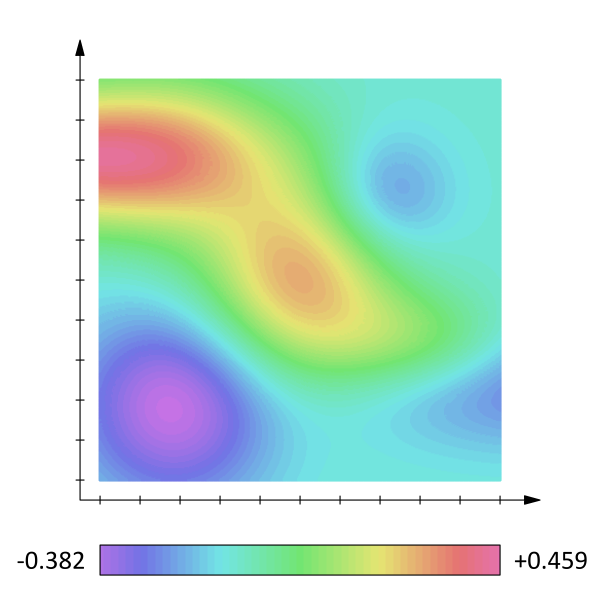
\includegraphics[width=0.7\textwidth]{Scalar_field.png} 
\caption{Scalar field,  \textit{Source: \textcircled{1}}}
\end{figure}
\end{column}
\end{columns}

} % END OF FRAME

\frame{
\frametitle{{Introduction - Vector Fields}}
\begin{columns}
\begin{column}{.5\textwidth}
\begin{itemize}
	\item visualized by a collection of arrows with a given magnitude and direction classically
	\bigskip
	\item Each position in space is mapped a scalar magnitude and an angle
	\bigskip
	\item Examples: flow field, magnetic field, gravitational field
\end{itemize}
\end{column}
\begin{column}{.5\textwidth}
\begin{figure}[t]
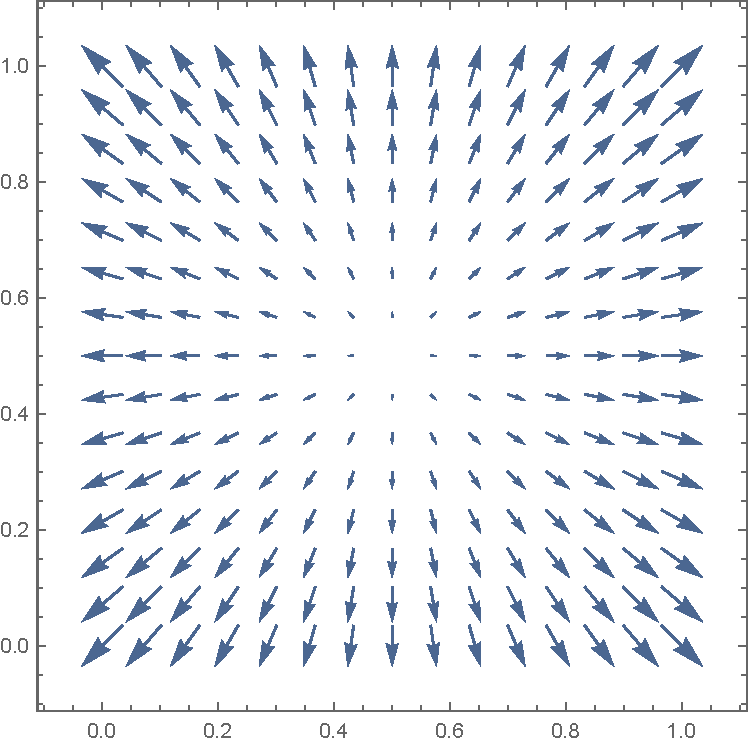
\includegraphics[width=0.4\textwidth]{vector_field.pdf} a)
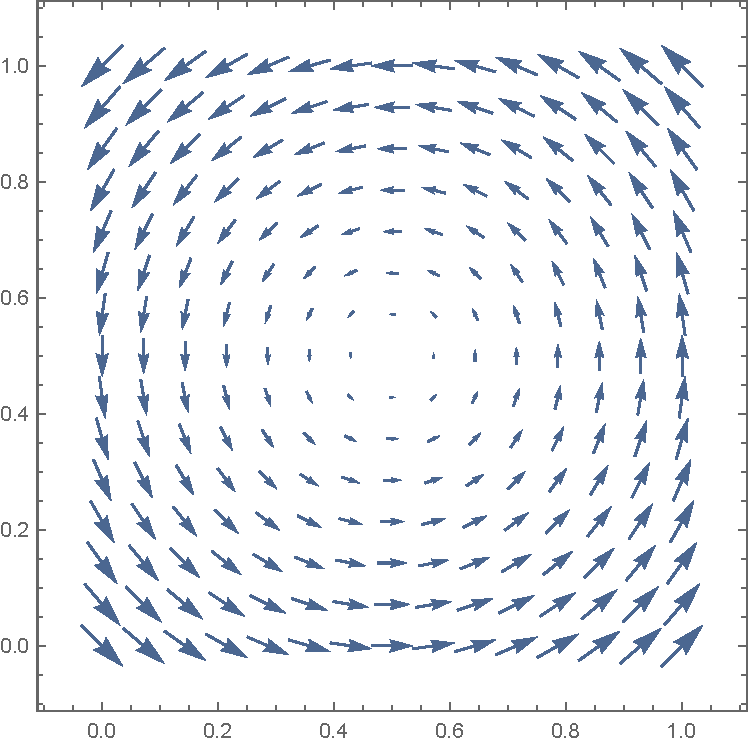
\includegraphics[width=0.4\textwidth]{vector_field2.pdf} b)
\caption{Vector fields: a) $\{x,y\}$, b) $\{-y,x\}$}
\end{figure}

\end{column}
\end{columns}

} % END OF FRAME

\frame{
\frametitle{{Introduction - Tensor Fields}}
\begin{columns}
\begin{column}{.5\textwidth}
\begin{itemize}
	\item Tensor fields are commonly visualized by:
	\begin{itemize}
		\item Glyphs
		\item Tensor field lines (TFLs)\\ $\Rightarrow$ Hyperstreamlines
	\end{itemize}
	\bigskip
	\item Each position in space is mapped a tensor describing a directional distribution
	\bigskip
	\item Scalar Measures: anisotropy index, tensor magnitude
\end{itemize}
\end{column}
\begin{column}{.5\textwidth}
\begin{figure}[t]
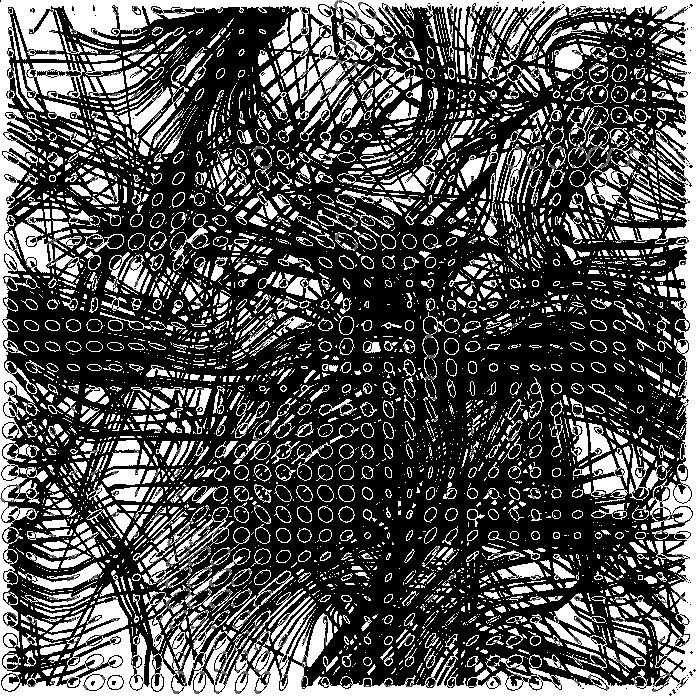
\includegraphics[width=0.4\textwidth]{random-global-TFL.png} a)
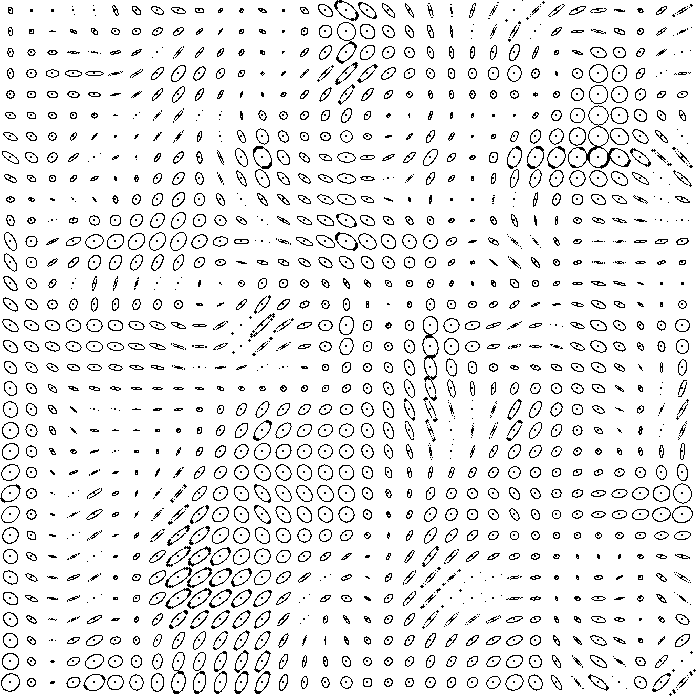
\includegraphics[width=0.4\textwidth]{random-global.png} b)
\caption{Tensor fields: a) Tensor field lines, b) Glyphs}
\end{figure}

\end{column}
\end{columns}

} % END OF FRAME

\frame{
\frametitle{{Glyphs}}
\begin{columns}
\begin{column}{.6\textwidth}
\begin{small}
\begin{itemize}
	\item glyphs are used to represent the principal component ellipsoid, i.e., the anisotropy characteristics and/or tensor magnitude
	\bigskip
	\item glyphs can be found in varying shapes, we define ellipsoids here for simplicity
\end{itemize}
\end{small}
\end{column}
\begin{column}{.4\textwidth}
\begin{figure}[t]
\centering
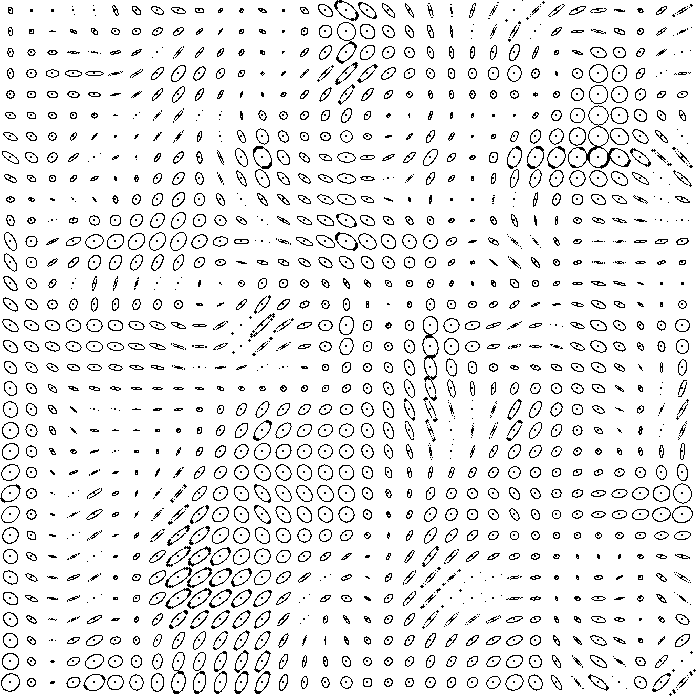
\includegraphics[height=0.9\textwidth]{random-global.png}
\caption{$2D$ glyphs for Random field}
\end{figure}

\end{column}
\end{columns}
} % END OF FRAME

\frame{
\frametitle{{Tensor Field Lines}}

\begin{columns}
\begin{column}{.6\textwidth}
\begin{small}
\begin{block}{\centering \textbf{Procedure}}
follow major/minor eigenvectors along pathlines
\end{block}
\end{small}
\bigskip
\begin{itemize}
	\item ambiguity for nearly isotropic cases: small changes in magnitude effect large changes in glyph orientation
	\item therefore susceptive to noise in data
\end{itemize}

\end{column}
\begin{column}{.4\textwidth}
\begin{figure}[t]
\centering
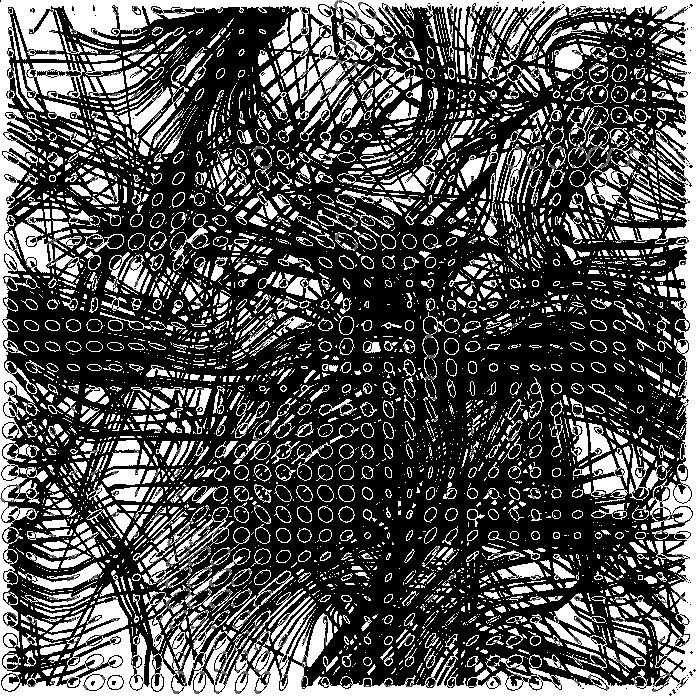
\includegraphics[height=0.9\textwidth]{random-global-TFL.png}
\caption{$2D$ glyphs and tensor field lines}
\end{figure}

\end{column}
\end{columns}
} % END OF FRAME

\frame{
\frametitle{{Introduction - Tensor Field Lines}}

\begin{figure}[!t]
\centering
  \begin{minipage}{0.22\textwidth}
      \centering
    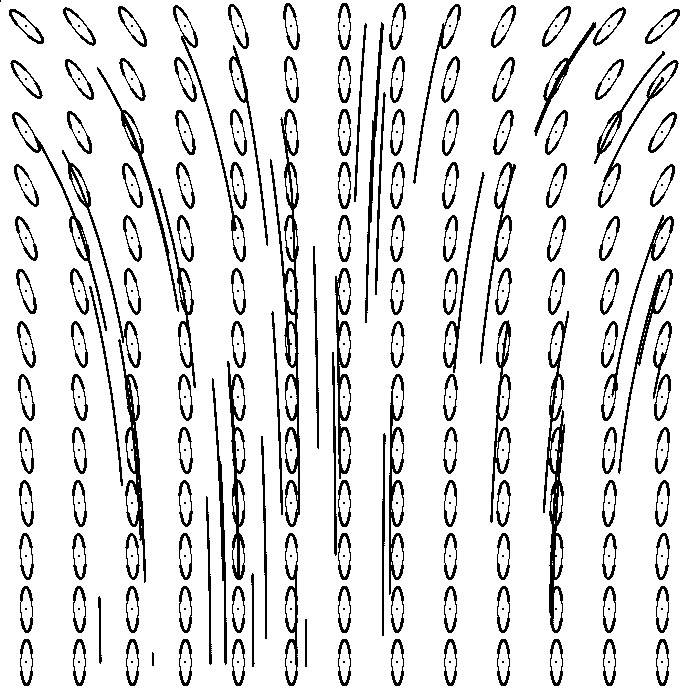
\includegraphics[height=\textwidth]{drain-TFL.png}
	a)
    \label{a)}
  \end{minipage}
  \begin{minipage}{0.22\textwidth}
      \centering
    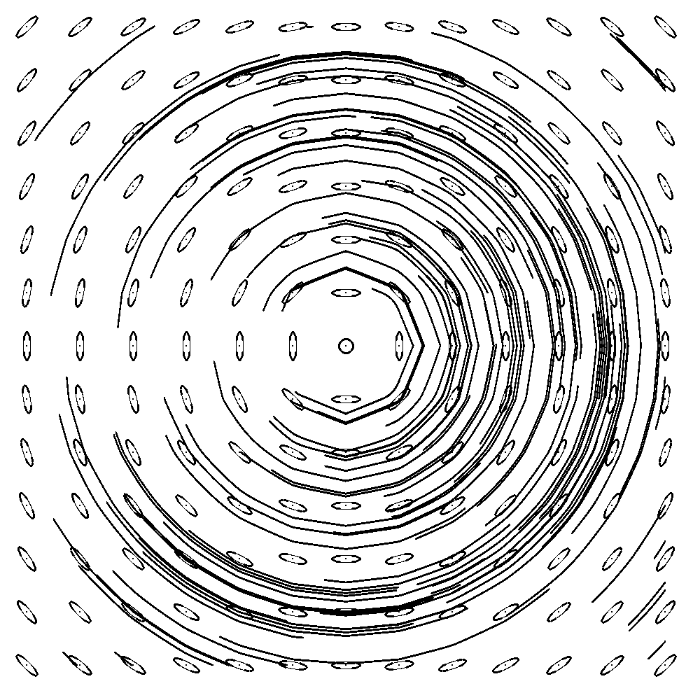
\includegraphics[height=\textwidth]{rings-TFL.png}
	b)
    \label{b)}
  \end{minipage}
  \begin{minipage}{0.22\textwidth}
      \centering
    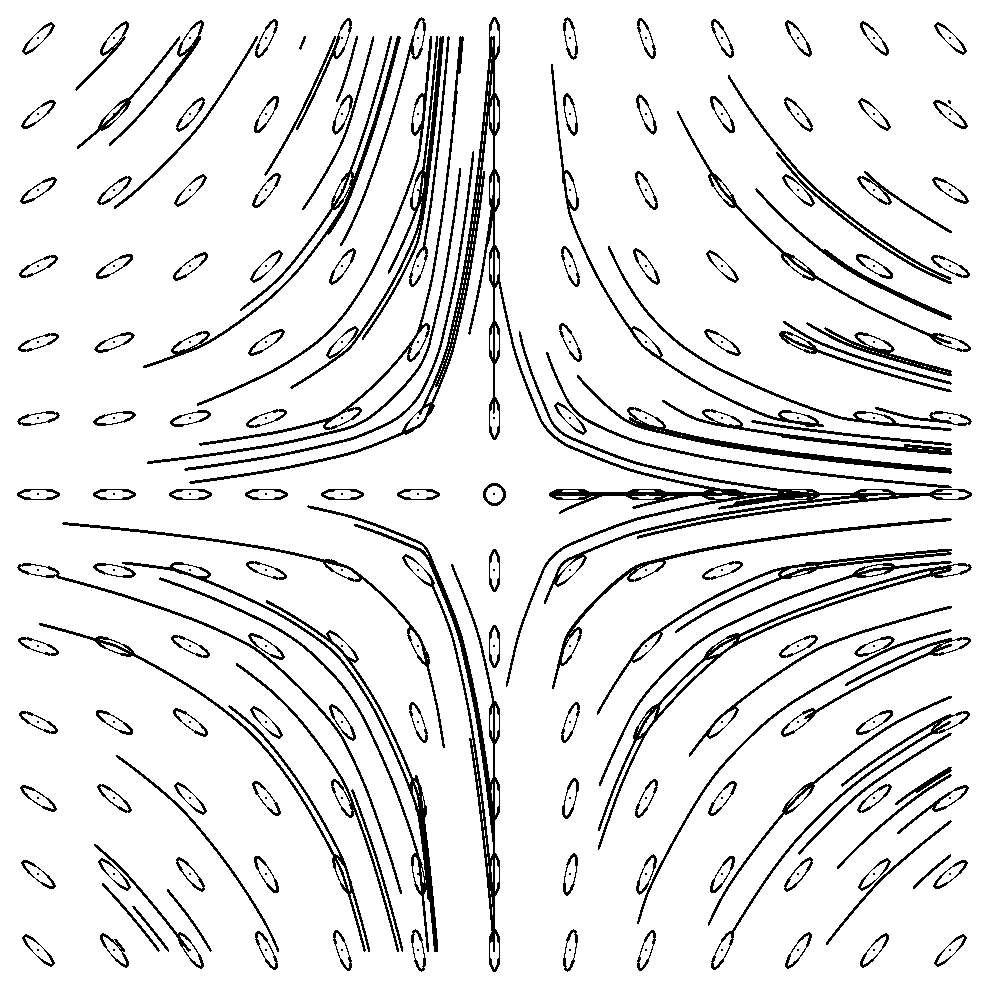
\includegraphics[height=\textwidth]{inverse-TFL.png}
	c)
    \label{b)}
  \end{minipage}
  \begin{minipage}{0.22\textwidth}
      \centering
    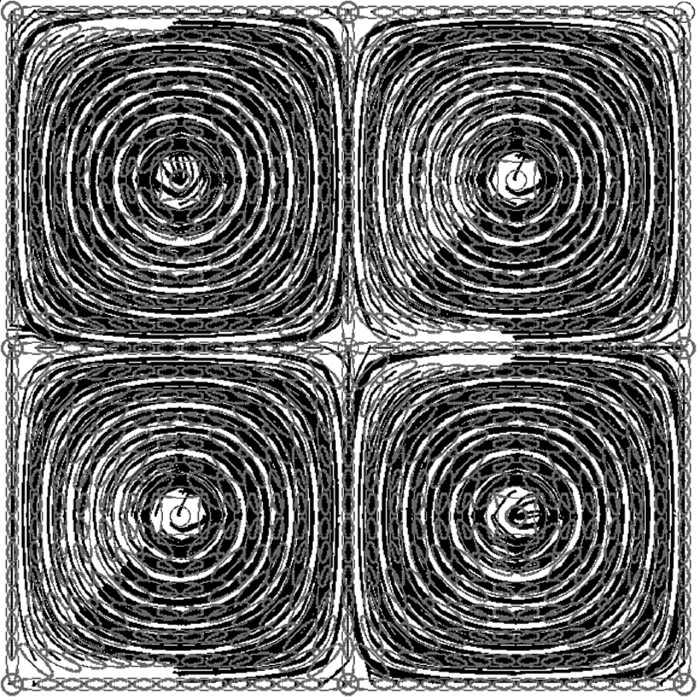
\includegraphics[height=\textwidth]{gyre-TFL.png}
	d)
    \label{b)}
  \end{minipage}
\caption{Several test fields: a)Drain, b) Rings, c) Inverse, d) Gyre}
\label{test_fields2}
\end{figure}

} % END OF FRAME}

%\frame{
%\frametitle{{Objectives}}
%
%\begin{itemize}
%	\item a light transport model (propagation scheme) following basic but crucial physical principles,
%	\item application of this model for tensor field visualization interpreting tensors as light transmission properties,
%	\item a FTLE (Finite-time Lyapunov exponents)-related approach called light transport gradient (LTG) for visualizing key structures, namely LCS (Lagrangian coherent structures) in 2D second-order tensor fields, and
%	\item application of our approach to both synthetic and real data involving brain and heart datasets.
%\end{itemize}
%
%} % END OF FRAME
%----------------------------------------

\subsection[Introduction]{Related Work}

\frame{
\frametitle{{Related Work - Global Illumination Methods}}
\begin{columns}
\begin{column}{.5\textwidth}
\begin{itemize}
	\item Discrete Ordinates Method
	\bigskip
	\item Lattice-Boltzmann method
	\bigskip
	\item Light Propagation Volumes
\end{itemize}
\end{column}
\begin{column}{.5\textwidth}
\begin{figure}[t]
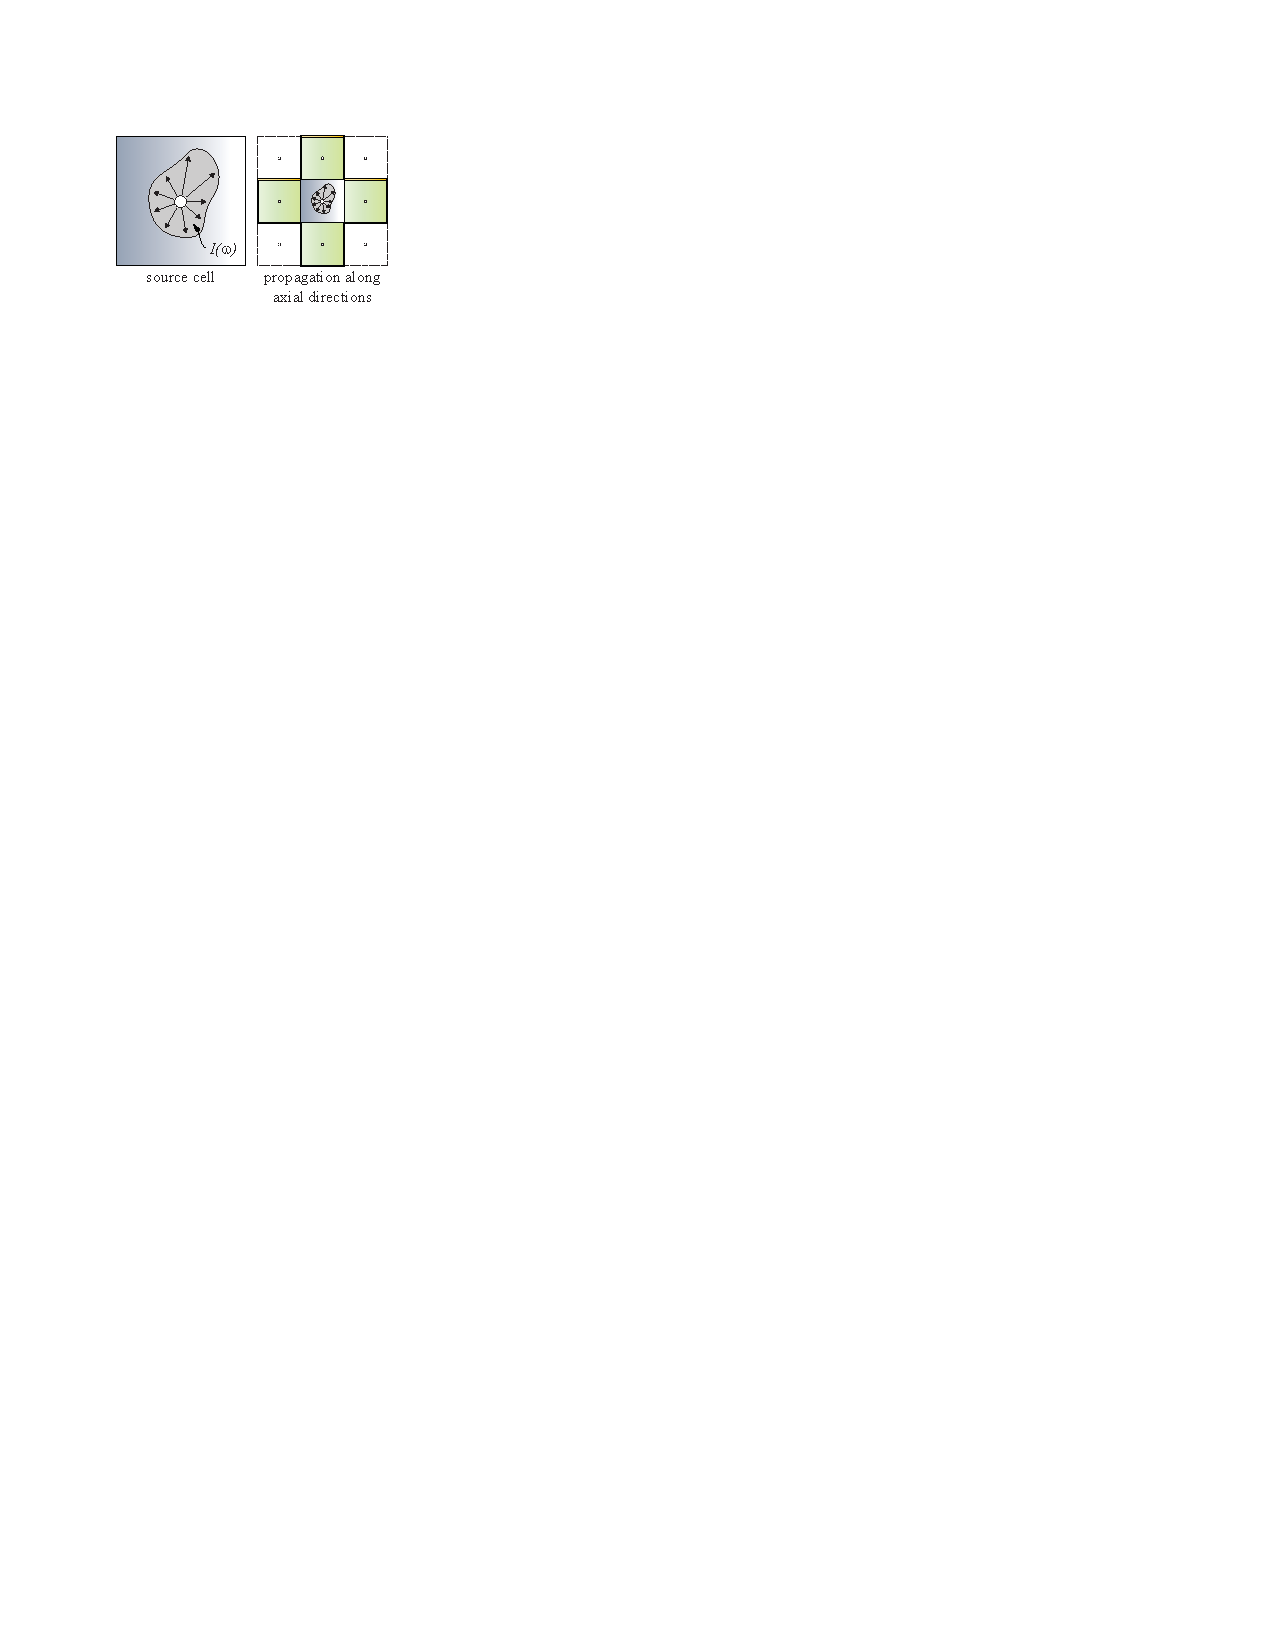
\includegraphics[width=0.55\textwidth]{LPV.pdf}
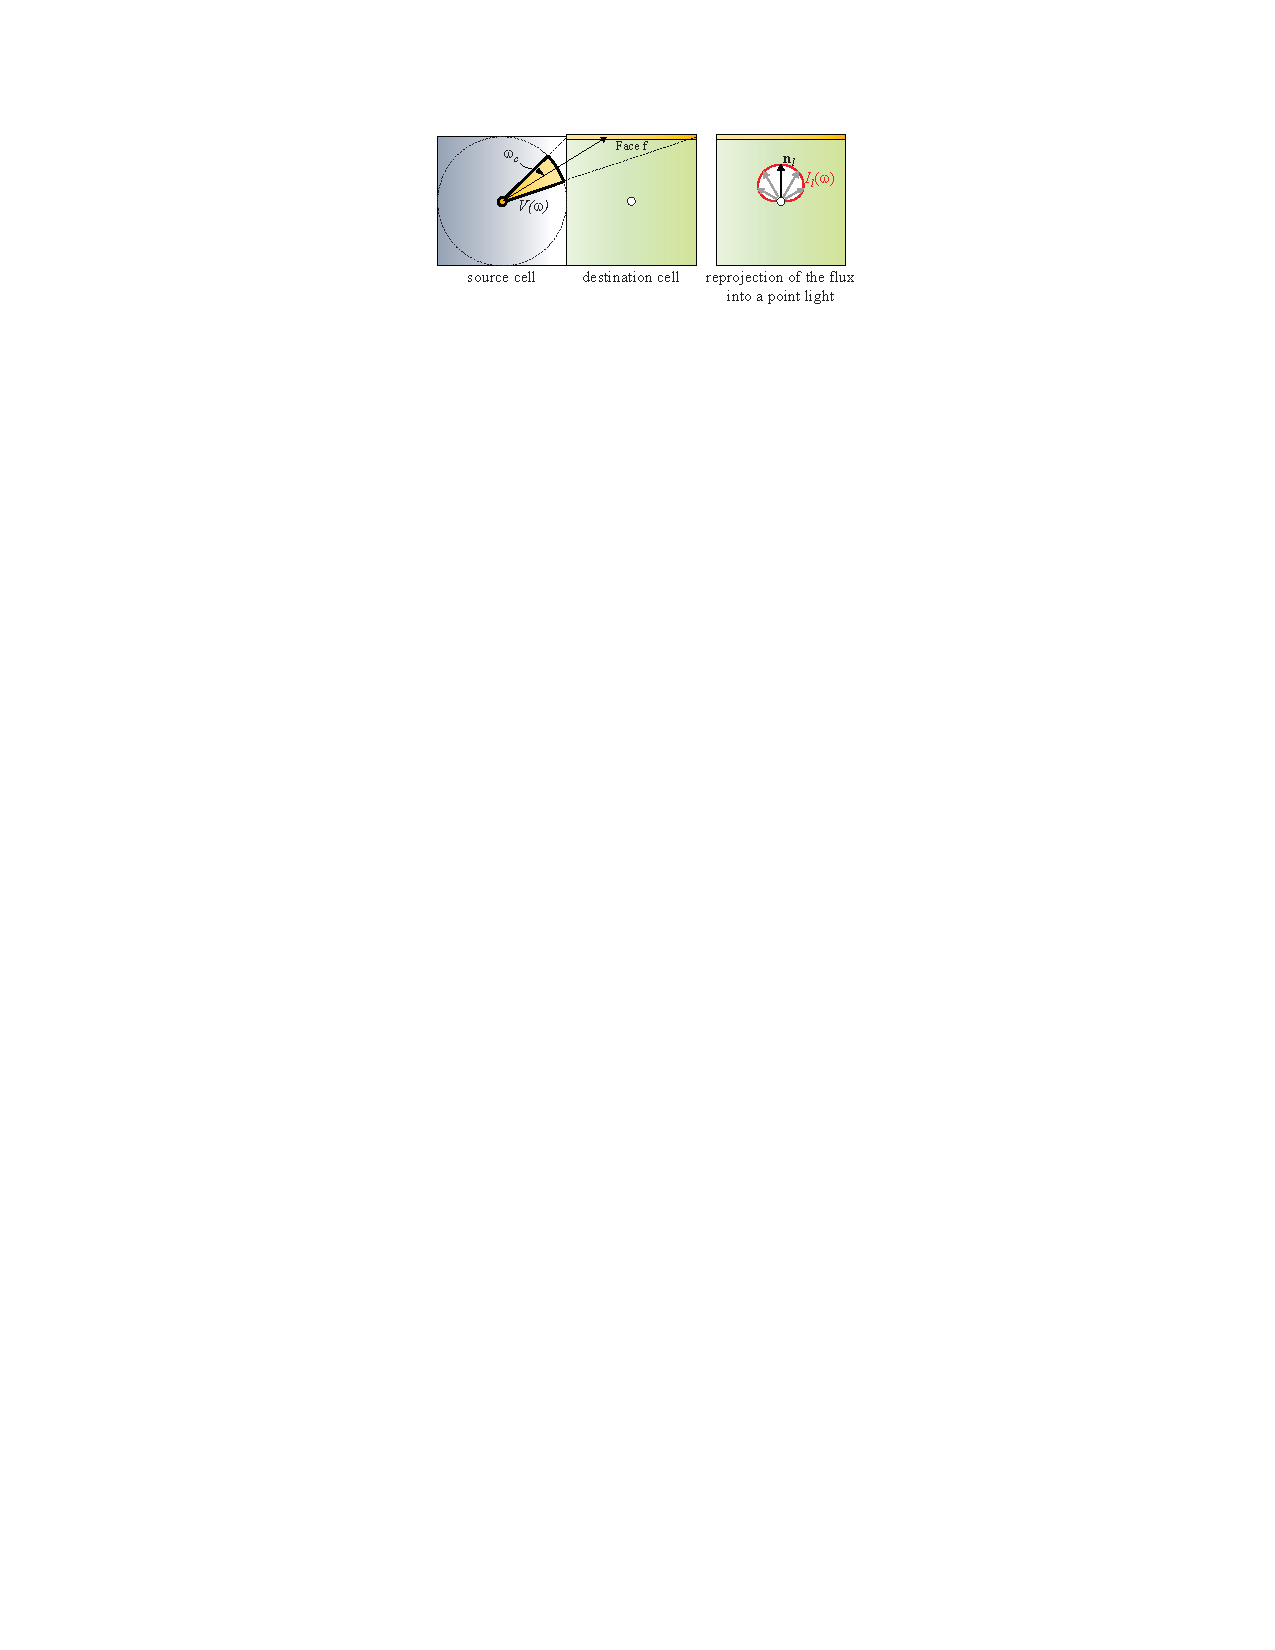
\includegraphics[width=0.55\textwidth]{LPV2.pdf} 
\caption{Light Propagation Volumes,  \textit{Source: \textcircled{1}}}
\end{figure}
\end{column}
\end{columns}

} % END OF FRAME

%\item Discrete Ordinates Method: discretizes RTE in both spatial and angular domain
%	\bigskip
%	\item Lattice-Boltzmann method: light propagation modeled as a diffusion process
%	\bigskip
%	\item Light Propagation Volumes: light exchanged between neighboring cells and stored locally

\frame{
\frametitle{{Related Work - Symmetric Tensor Field Visualization}}

\begin{itemize}
	\item Glyphs: represent anisotropy with shape and orientation
	\item Tensor Field Lines (TFLs): follow the eigenvector along tensor field lines
	\item Tensorlines: introduce artificial inertia on TFLs to increase stability
	\item HyperLIC: use Line Integral Convolution from Vector Field Visualization on TFLs
	\item FTLE: exploit the gradient of the flow map of TFLs to generate an FTLE field
	\item Scalar Measures: tensor magnitude, diffusivity, fractional anisotropy, anisotropy coefficients (measures)
\end{itemize}


} % END OF FRAME

\frame{
\frametitle{{Related Work - Asymmetric Tensor Field Visualization}}

\begin{itemize}
	\item Dual Eigenvectors: use complex conjugate eigenvectors as co-visualization for the complex domain along with ordinary eigenvectors to represent the real domain
	\bigskip
	\item Pseudo Eigenvectors: extension for dual eigenvectors to a full set or graph
	\bigskip
	\item Scalar Measures: tensor magnitude, tensor mode, isotropy index
\end{itemize}


} % END OF FRAME
%----------------------------------------


%----------------------------------------

%======================================== END OF SECTION
\subsection[Introduction]{Motivation}
\frame{
\frametitle{{Motivation - Tensor Fields}}
\begin{figure}[!t]
\centering
  \begin{minipage}{0.3\textwidth}
      \centering
    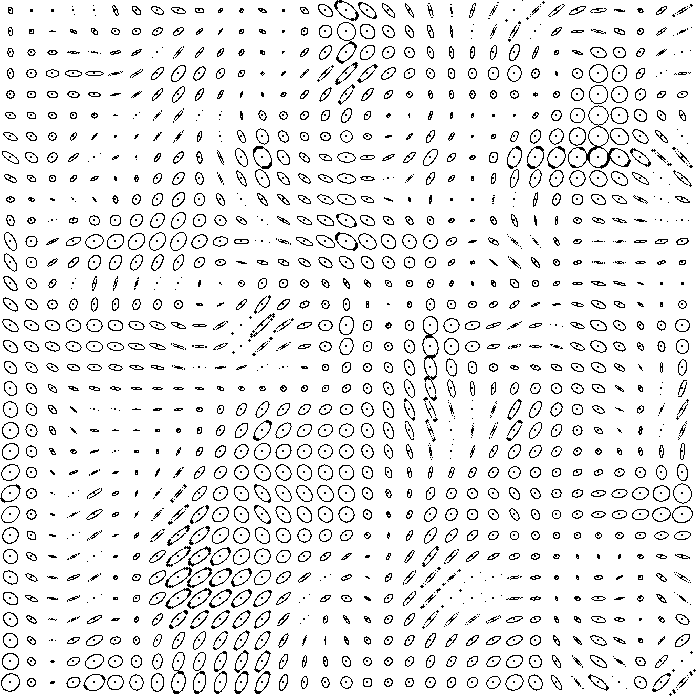
\includegraphics[height=0.7\textwidth]{random-global.png}
	a)
    \label{a)}
  \end{minipage}
  \begin{minipage}{0.3\textwidth}
      \centering
    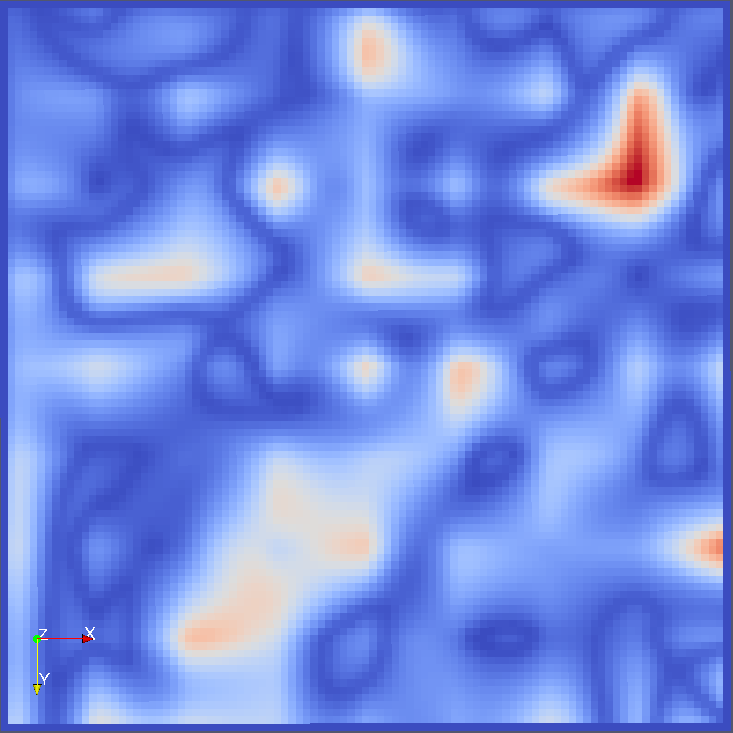
\includegraphics[height=0.7\textwidth]{random_global.png}
	b)
    \label{b)}
  \end{minipage}
  \begin{minipage}{0.3\textwidth}
      \centering
    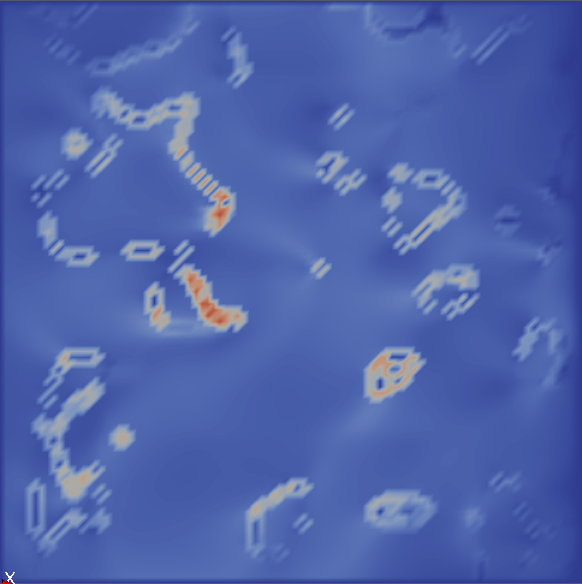
\includegraphics[height=0.7\textwidth]{random_local_slice0.png}
	c)
    \label{b)}
  \end{minipage}
\caption{Random field: a) field, b) tensor magnitude, c) FTLE}
\label{test_fields2}
\end{figure}
Applications:
\begin{itemize}
	\item Vector fields: describe spatial gradient called Jacobian-matrix,
	\item Fluid and solid continuum mechanics: stress tensor (e.g. Cauchy stress tensor)
	\item DT-MRI: diffusion tensor - magnetic resonance imaging
\end{itemize}
} % END OF FRAME

%\item Vector fields: to describe the directionally dependent spatial gradient called Jacobian-matrix,
%	\item Fluid and solid continuum mechanics: to describe a whole distribution of stresses
%	\item DT-MRI: diffusion tensor - magnetic resonance imaging: to describe the diffusion characteristics of water molecules within tissue

\section[Fundamentals]{Fundamentals}

\frame{
\frametitle{{Fundamentals}}

\begin{block}{\centering \textbf{Tensor Fields}}
\begin{itemize}
	\item order-$o$ generalization of a matrix with indices of run length $n$ for $n\times n$ matrices
	\item number arrays following covariant or contravariant transformation rules
	\item represenation needed for a whole directional distribution for each point in space
\end{itemize}
\end{block}
\begin{table}[b]
\centering
\caption{Tensor Shapes}\bigskip
 \begin{tabular}{c|c|c|c|c|c|c}
\textbf{order} & 0 & 1 & 2 & 3 & ... & o \\ 
\hline 
\textbf{shape} & scalar & vector & matrix & ``3D matrix'' & ... & order-$o$ matrix\\ 
\end{tabular}
\label{tensor}
 \end{table} 
} % END OF FRAME

\frame{
\frametitle{{Fundamentals}}

\begin{columns}
\begin{column}{.5\textwidth}
\begin{block}{\centering \textbf{Cauchy stress tensor}}
\begin{itemize}
	\item classical physical example of a tensor
	\item consistent of $3$ stress vectors arranged in row-major order
	\item maps an incoming direction vector $\mathbf{n}$ a resulting stress vector $\mathbf{T^{(n)}} = \mathbf{n}\cdot\boldsymbol{\sigma}$ per transformation
\end{itemize}

\end{block}
\end{column}
\begin{column}{.5\textwidth}
\begin{figure}[t]
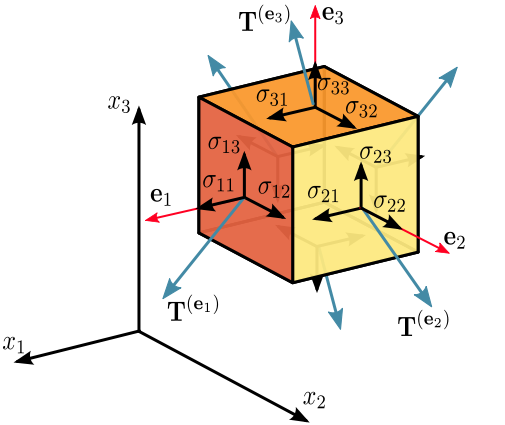
\includegraphics[width=0.5\textwidth]{stress_tensor.png} 
\caption{Cauchy stress tensor,  \textit{Source: \textcircled{2}}}
\end{figure}
\end{column}
\end{columns}

} % END OF FRAME

%\item classical physical example of a tensor
%	\item consistent of $3$ stress vectors arranged in row-major order
%	\item these represent the magnitude and orientation of the resulting stress at plane $x,y,z$ in direction $x,y,z$
%	\item maps an incoming direction vector $\mathbf{n}$ a resulting stress vector $\mathbf{T^{(n)}} = \mathbf{n}\cdot\boldsymbol{\sigma}$ per transformation

\frame{
\frametitle{{Polar Coordinates}}

\begin{columns}
\begin{column}{.5\textwidth}
\begin{block}{\centering \textbf{Conversion Formulas}}
Polar$\mapsto$Cartesian
\begin{align*}
	x &= r \cos \omega, \\
 	y &= r \sin \omega.
\end{align*}
Cartesian$\mapsto$Polar
\begin{align*}
	r &= \sqrt{x^2 + y^2}, \\
\omega &= \operatorname{atan2}(y, x).
\end{align*}

\end{block}
\end{column}
\begin{column}{.5\textwidth}
\begin{figure}[t]
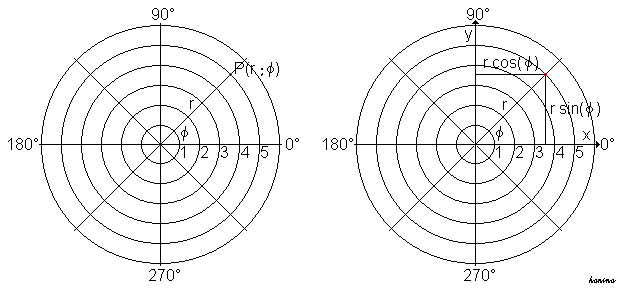
\includegraphics[width=0.7\textwidth]{polarkoordinaten.png}
\caption{Polar coordinates,  \textit{Source: \textcircled{3}}}
\end{figure}
\bigskip
\begin{itemize}
	\item polar function $f: \omega\mapsto r$ maps each angle $\omega$ a magnitude $r(\omega)$
\end{itemize}
\end{column}
\end{columns}

} % END OF FRAME

\frame{
\frametitle{{Principal Component Analysis}}

\begin{columns}
\begin{column}{.6\textwidth}
\begin{small}
\begin{block}{\centering \textbf{Matrix Decompositions}}
Eigenvalue Decomposition: 
$
	\mathbf{A} = \mathbf{R}\mathbf{S}\mathbf{R}^*
$\\
Singular Value Decomposition (SVD): 
$
	\mathbf{A} = \mathbf{U} \mathbf{\Sigma} \mathbf{V}^*
$
\end{block}
\end{small}
\bigskip
\begin{itemize}
	\item used to determine the main directions of variance (principal components) in stochastic data
	\item used to determine the subsequent base transformations composing affine transformations
\end{itemize}

\end{column}
\begin{column}{.4\textwidth}
\begin{figure}[t]
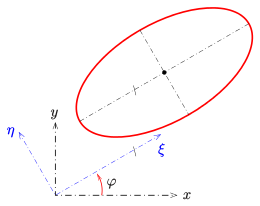
\includegraphics[width=0.7\textwidth]{HAT.png}
\caption{Principal component analysis,  \textit{Source: \textcircled{4}}}
\end{figure}

\end{column}
\end{columns}
} % END OF FRAME


\frame{
\frametitle{{Principal Component Analysis}}


\includemovie{0.49\textwidth}{0.4\textwidth}{scale.swf}
\includemovie{0.49\textwidth}{0.4\textwidth}{rotate.swf}


} % END OF FRAME

\frame{
\frametitle{{Finite-Time Lyapunov exponents}}

\begin{columns}
\begin{column}{.6\textwidth}
\begin{small}
\begin{block}{\centering \textbf{Definition}}
Local: 
$
	\sigma = \frac{1}{\lvert T\rvert}\ln \frac{\Delta}{\delta}
$\\
Global: 
$
	\sigma(\mathbf{x})=\frac{1}{\lvert T\rvert}\ln \|\nabla\mathbf{\upvarphi(x)}\|_2
$\\
{\scriptsize whereas $\| A\| _2 = \sqrt{\lambda_{max}(A^TA)}$ is the spectral norm of matrix $A$}
\end{block}
\end{small}
\begin{itemize}
	\item measure for separation abilities of time-dependent dynamical systems concerning massless tracer particles
	\item in particular concerning Lagrangian view in vector fields: placing two close-by particles into and moving with the flow
\end{itemize}

\end{column}
\begin{column}{.4\textwidth}
\begin{figure}[t]
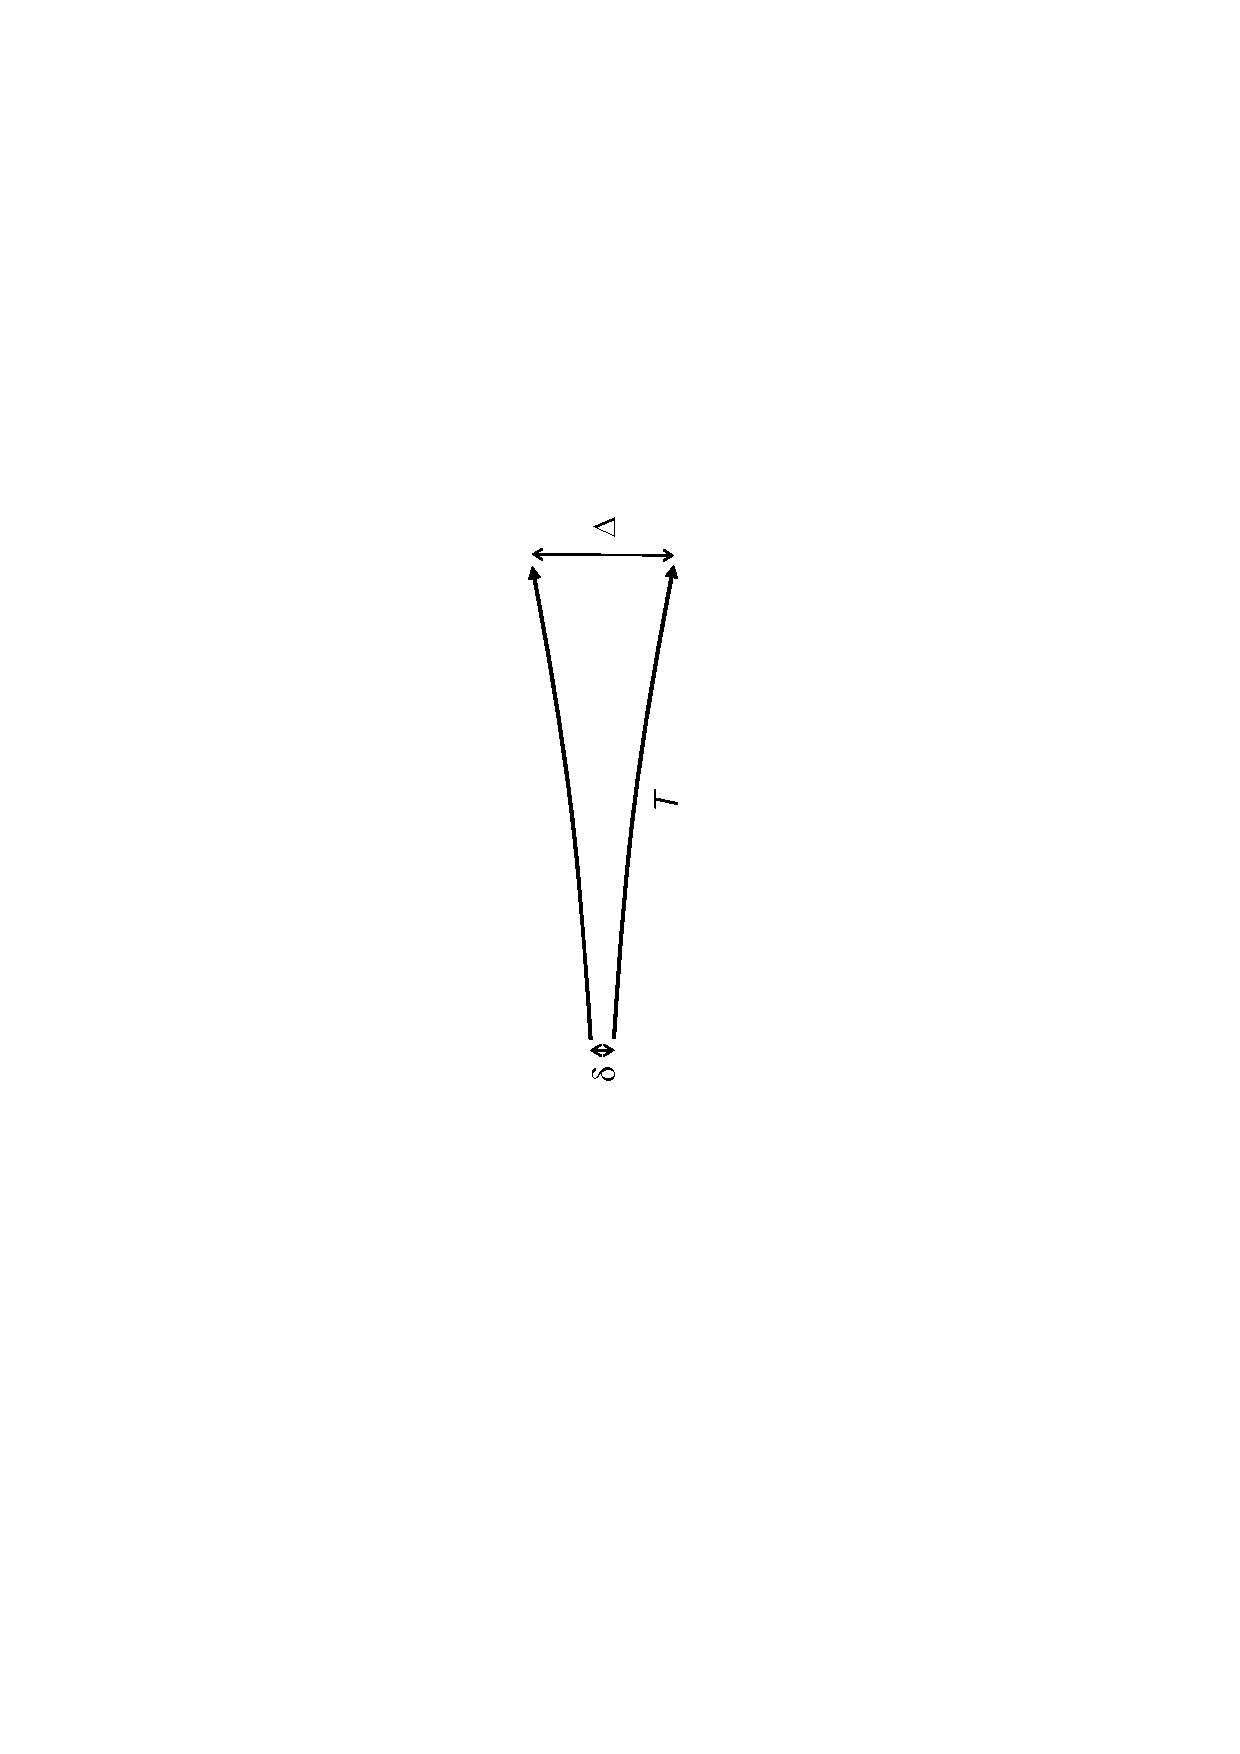
\includegraphics[height=0.9\textwidth]{ftle_sep.pdf}
\caption{Path line separation,  \textit{Source: \textcircled{4}}}
\end{figure}

\end{column}
\end{columns}
} % END OF FRAME

%
%\frame{
%\frametitle{{Symmetric Tensor Fields}}
%
%\begin{figure}[!t]
%\centering
%  \begin{minipage}{0.4\textwidth}
%    \centering
%    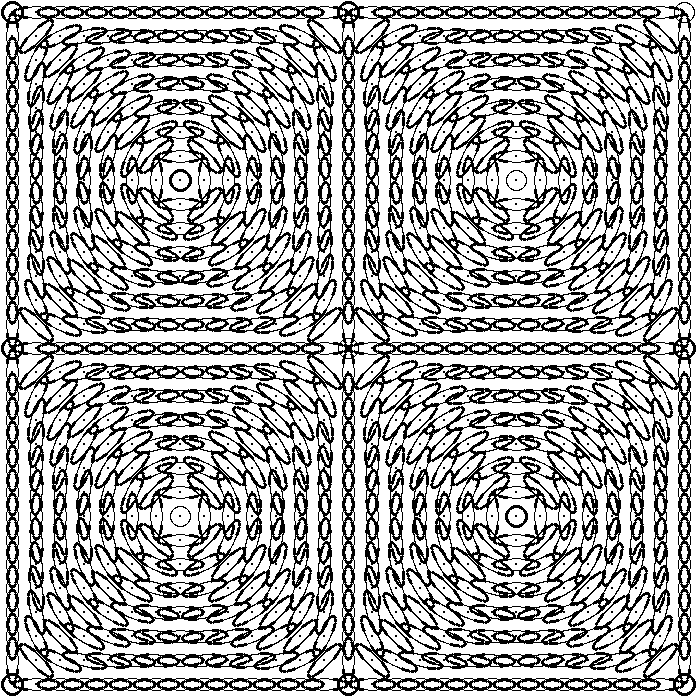
\includegraphics[width=0.8\textwidth]{gyre.png}
%	a)
%    \label{a)}
%  \end{minipage}
%  \begin{minipage}{0.4\textwidth}
%    \centering
%    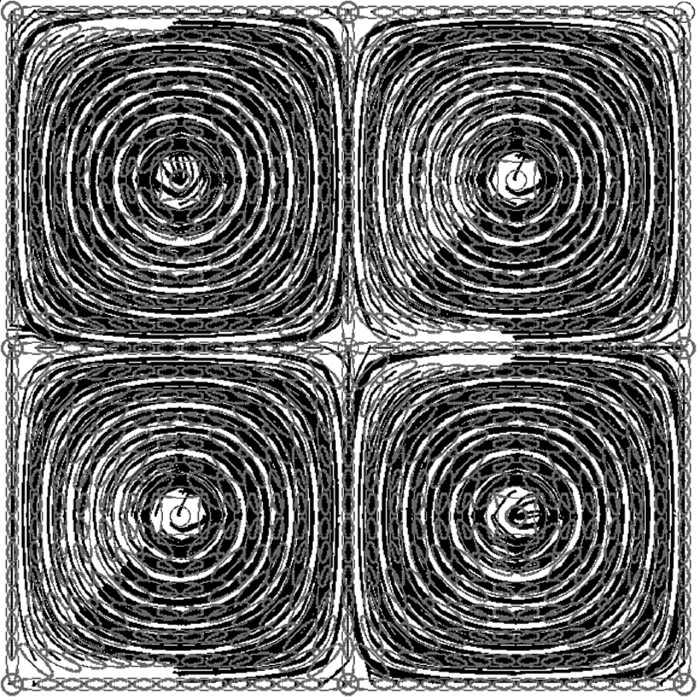
\includegraphics[width=0.8\textwidth]{gyre-TFL.png}
%	b)
%    \label{b)}
%  \end{minipage}
%\caption{Gyre test field: a) glyphs, b) tensor field lines for a)}
%\label{gyre}
%\end{figure}
%
%} % END OF FRAME
%
%\frame{
%\frametitle{{Asymmetric Tensor Fields}}
%
%\begin{figure}[!t]
%\centering
%  \begin{minipage}{0.23\textwidth}
%  \centering
%    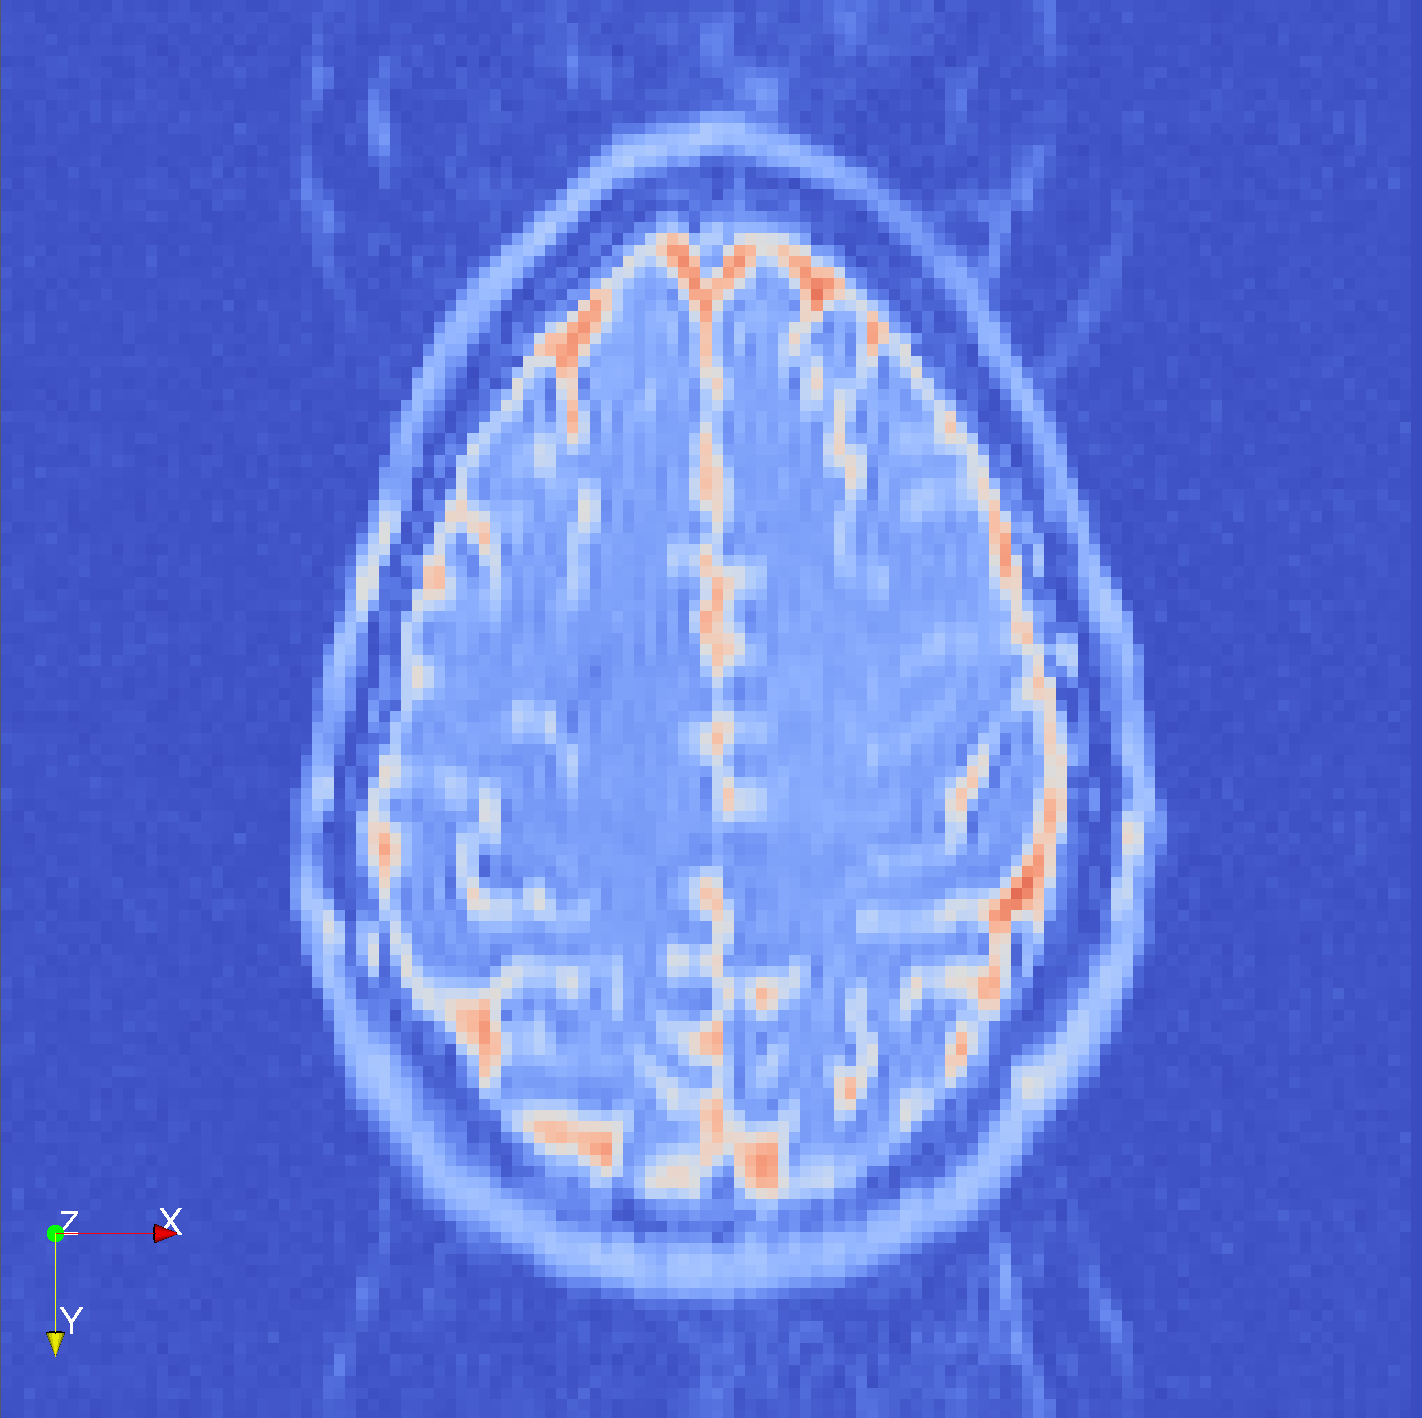
\includegraphics[height=\textwidth]{brain_org.png}
%    \label{a)}
%	a)
%  \end{minipage}
%  \begin{minipage}{0.23\textwidth}
%  \centering
%    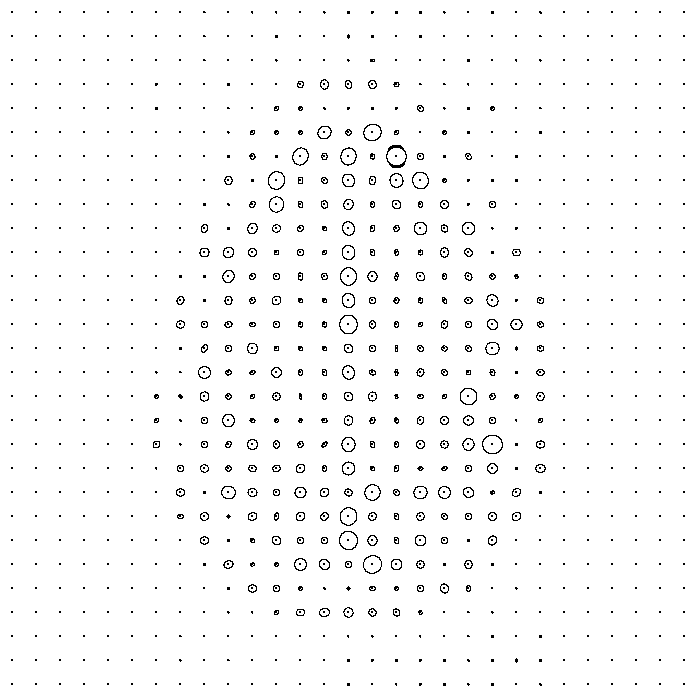
\includegraphics[height=\textwidth]{brainDwnsmpl.png}
%    \label{b)}
%    b)
%  \end{minipage}
%  \begin{minipage}{0.23\textwidth}
%  \centering
%    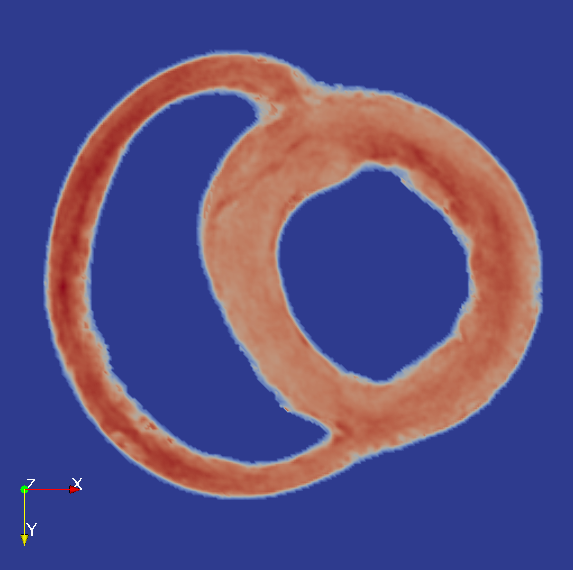
\includegraphics[height=\textwidth]{heart_org.png}
%    \label{b)}
%    a)
%  \end{minipage}
%  \begin{minipage}{0.23\textwidth}
%  \centering
%    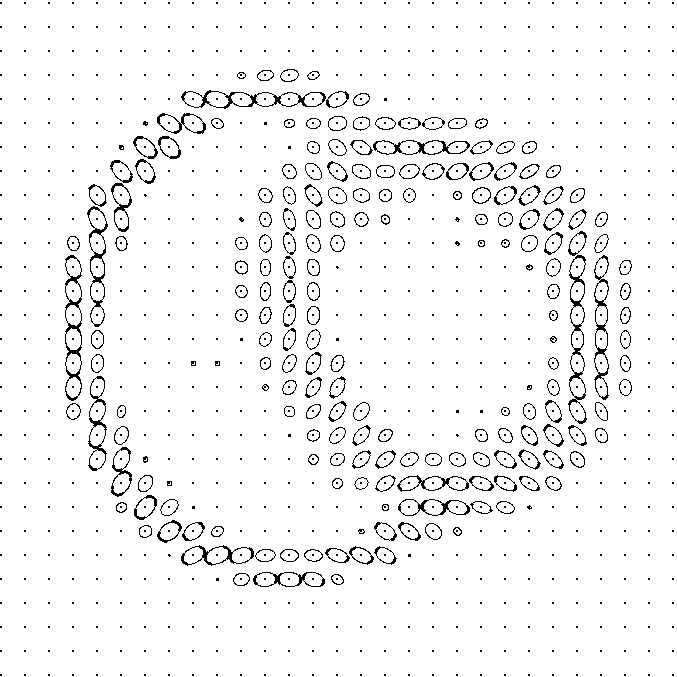
\includegraphics[height=\textwidth]{heartDwnsmpl.png}
%    \label{b)}
%    b)
%  \end{minipage}
%\caption{Brain and Heart dataset: a) tensor magnitude, b) ellipsoid glyphs}
%\label{real1}
%\end{figure}
%
%} % END OF FRAME

\section[Method]{Method}

\frame{
\frametitle{{Propagation Scheme}}

\begin{columns}
\begin{column}{.6\textwidth}
\begin{itemize}
	\item light propagation scheme exchanging energies between neighboring cells
	\item propagates intensities from initially set cells to corresponding neighbors
	\item eventually to model anisotropy characteristics of tensor field on top
\end{itemize}

\end{column}
\begin{column}{.4\textwidth}
\begin{figure}[!t]
  \centering
 {
    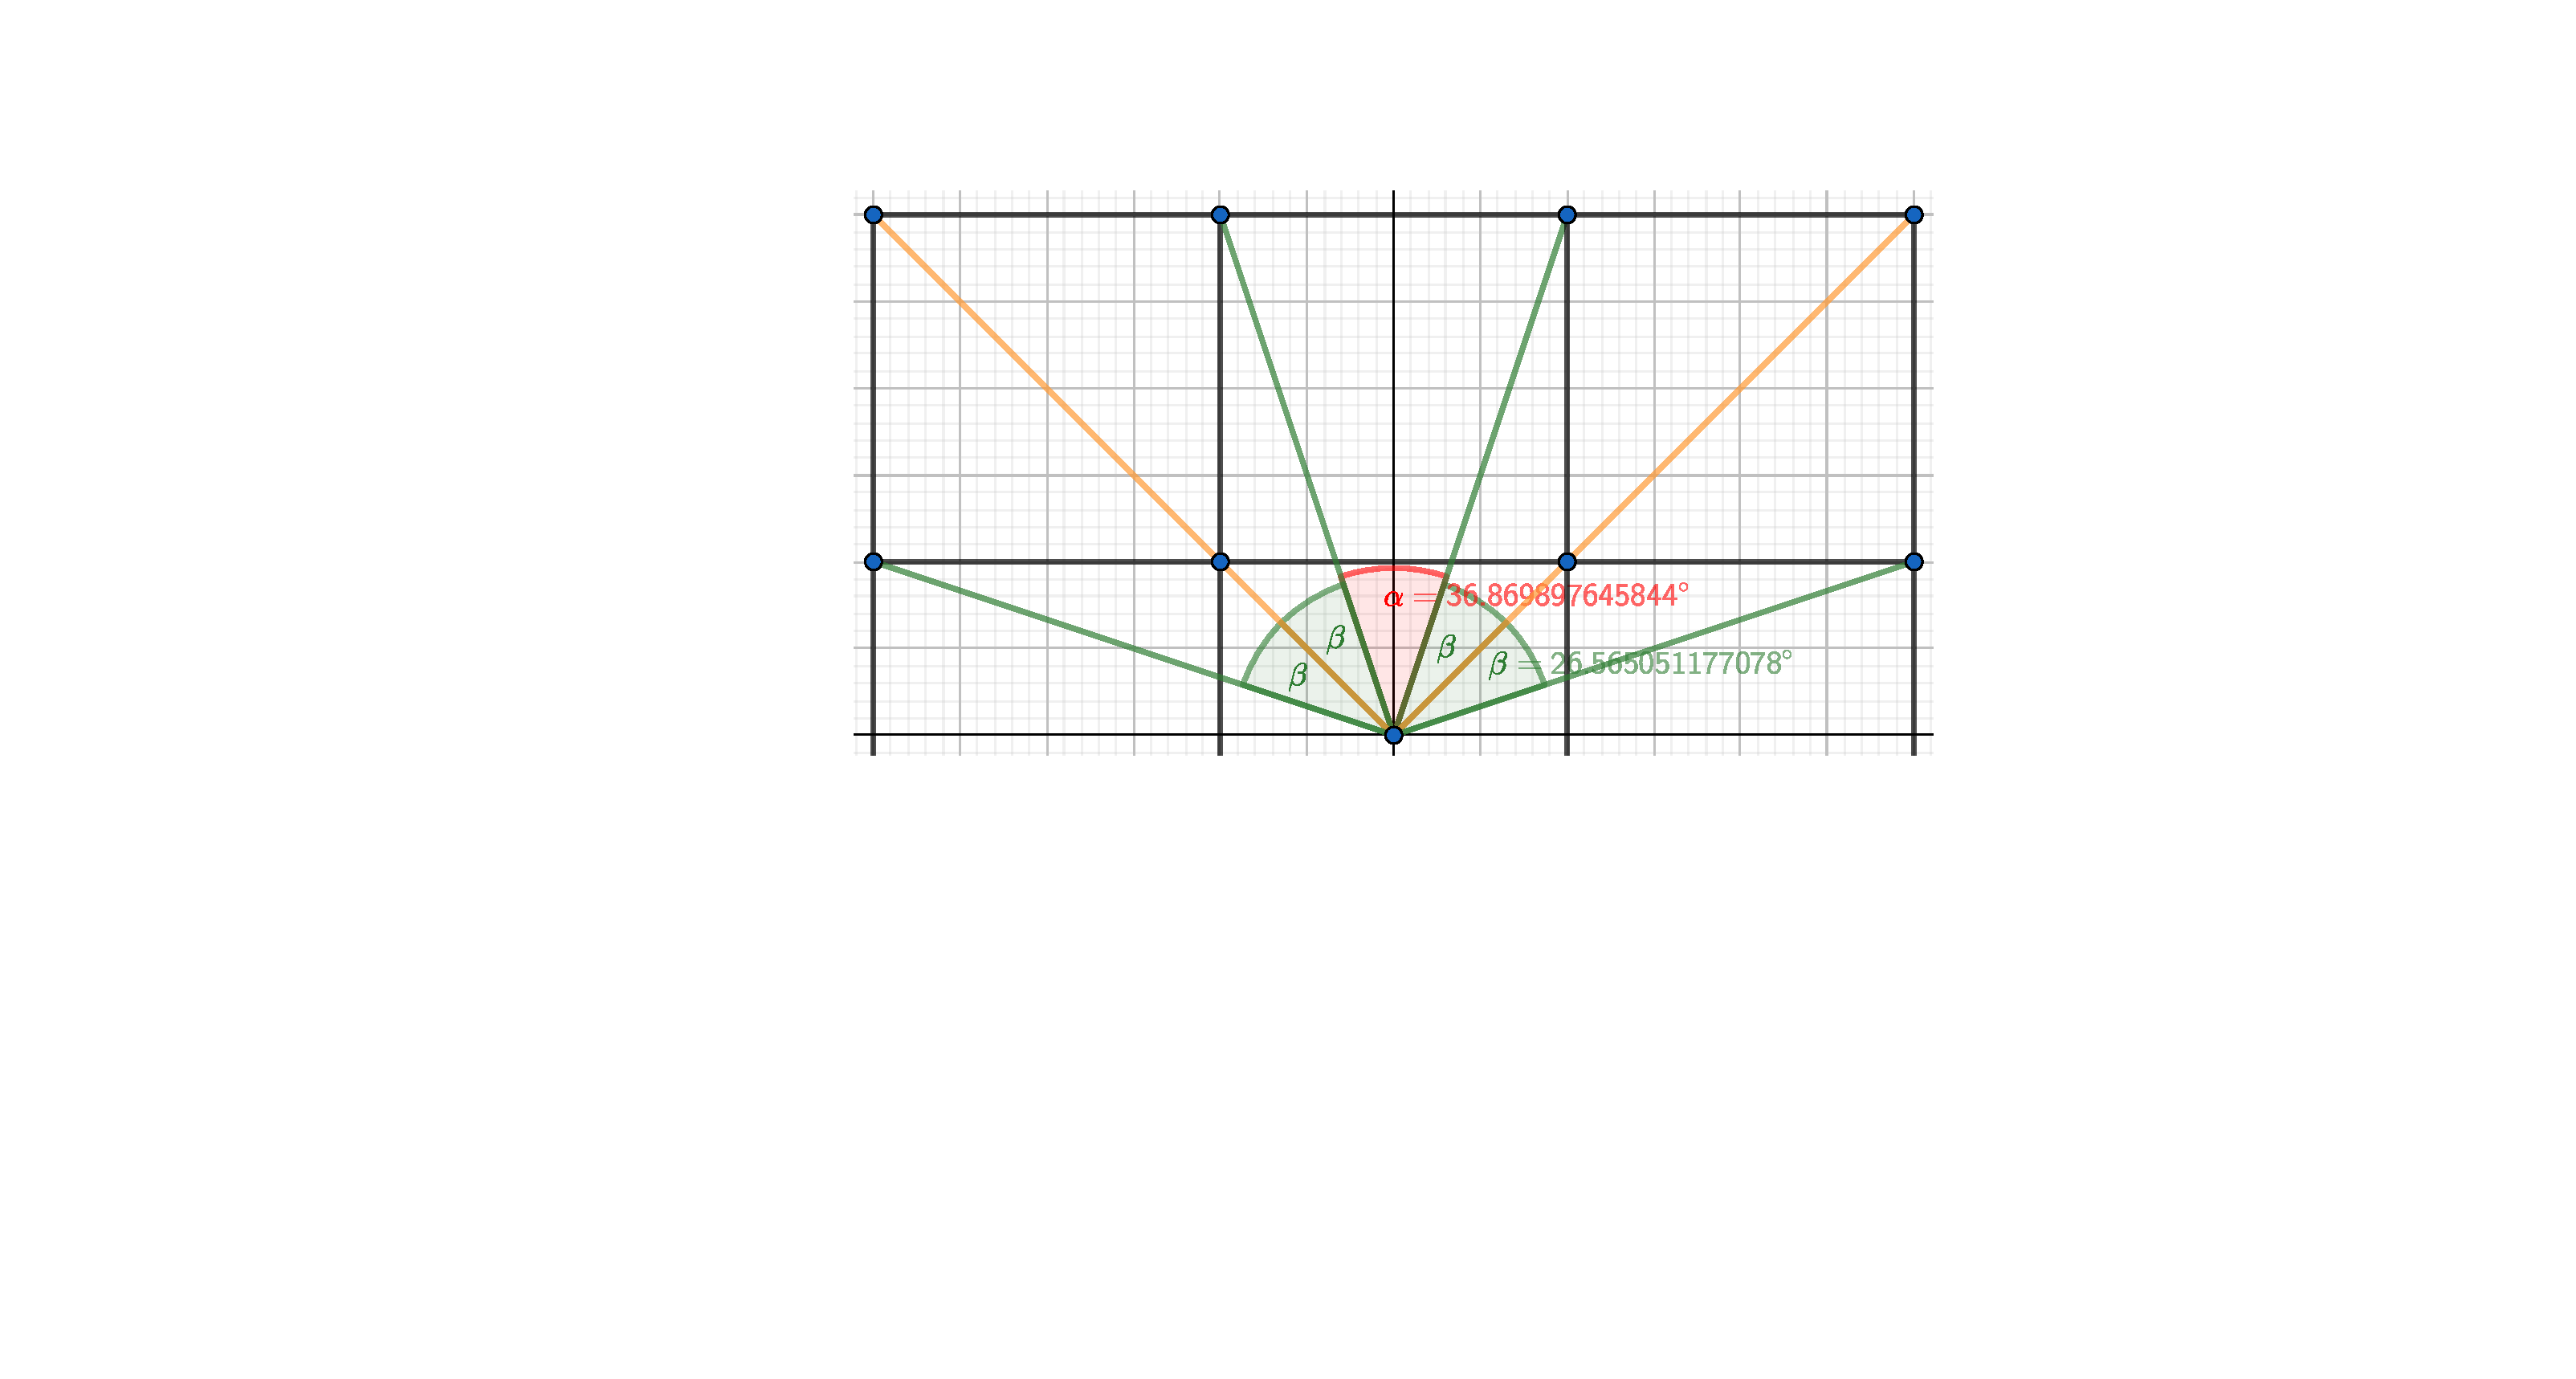
\includegraphics[width=\textwidth]
    {geogebra-export_large.pdf}
  }
  \caption{Propagation Scheme}
  \label{scheme}
\end{figure}

\end{column}
\end{columns}
} % END OF FRAME

\frame{
\frametitle{{Propagation Scheme}}

\begin{columns}
\begin{column}{.6\textwidth}
\begin{align*}
	\varepsilon_\alpha &= \frac{\frac{\beta}{\alpha+2\beta}}{\frac{\beta}{\alpha+2\beta} + \frac{\beta}{2\beta}} \approx 0.362291\\
	\varepsilon_\beta &= \frac{\frac{\beta}{2\beta}}{\frac{\beta}{\alpha+2\beta} + \frac{\beta}{2\beta}} \approx 0.63771\\
	\Phi_{t} &= \varepsilon_k\int I(\omega)\mathop{d\omega}
\end{align*}

\end{column}
\begin{column}{.4\textwidth}
\begin{figure}[!t]
  \centering
 {
    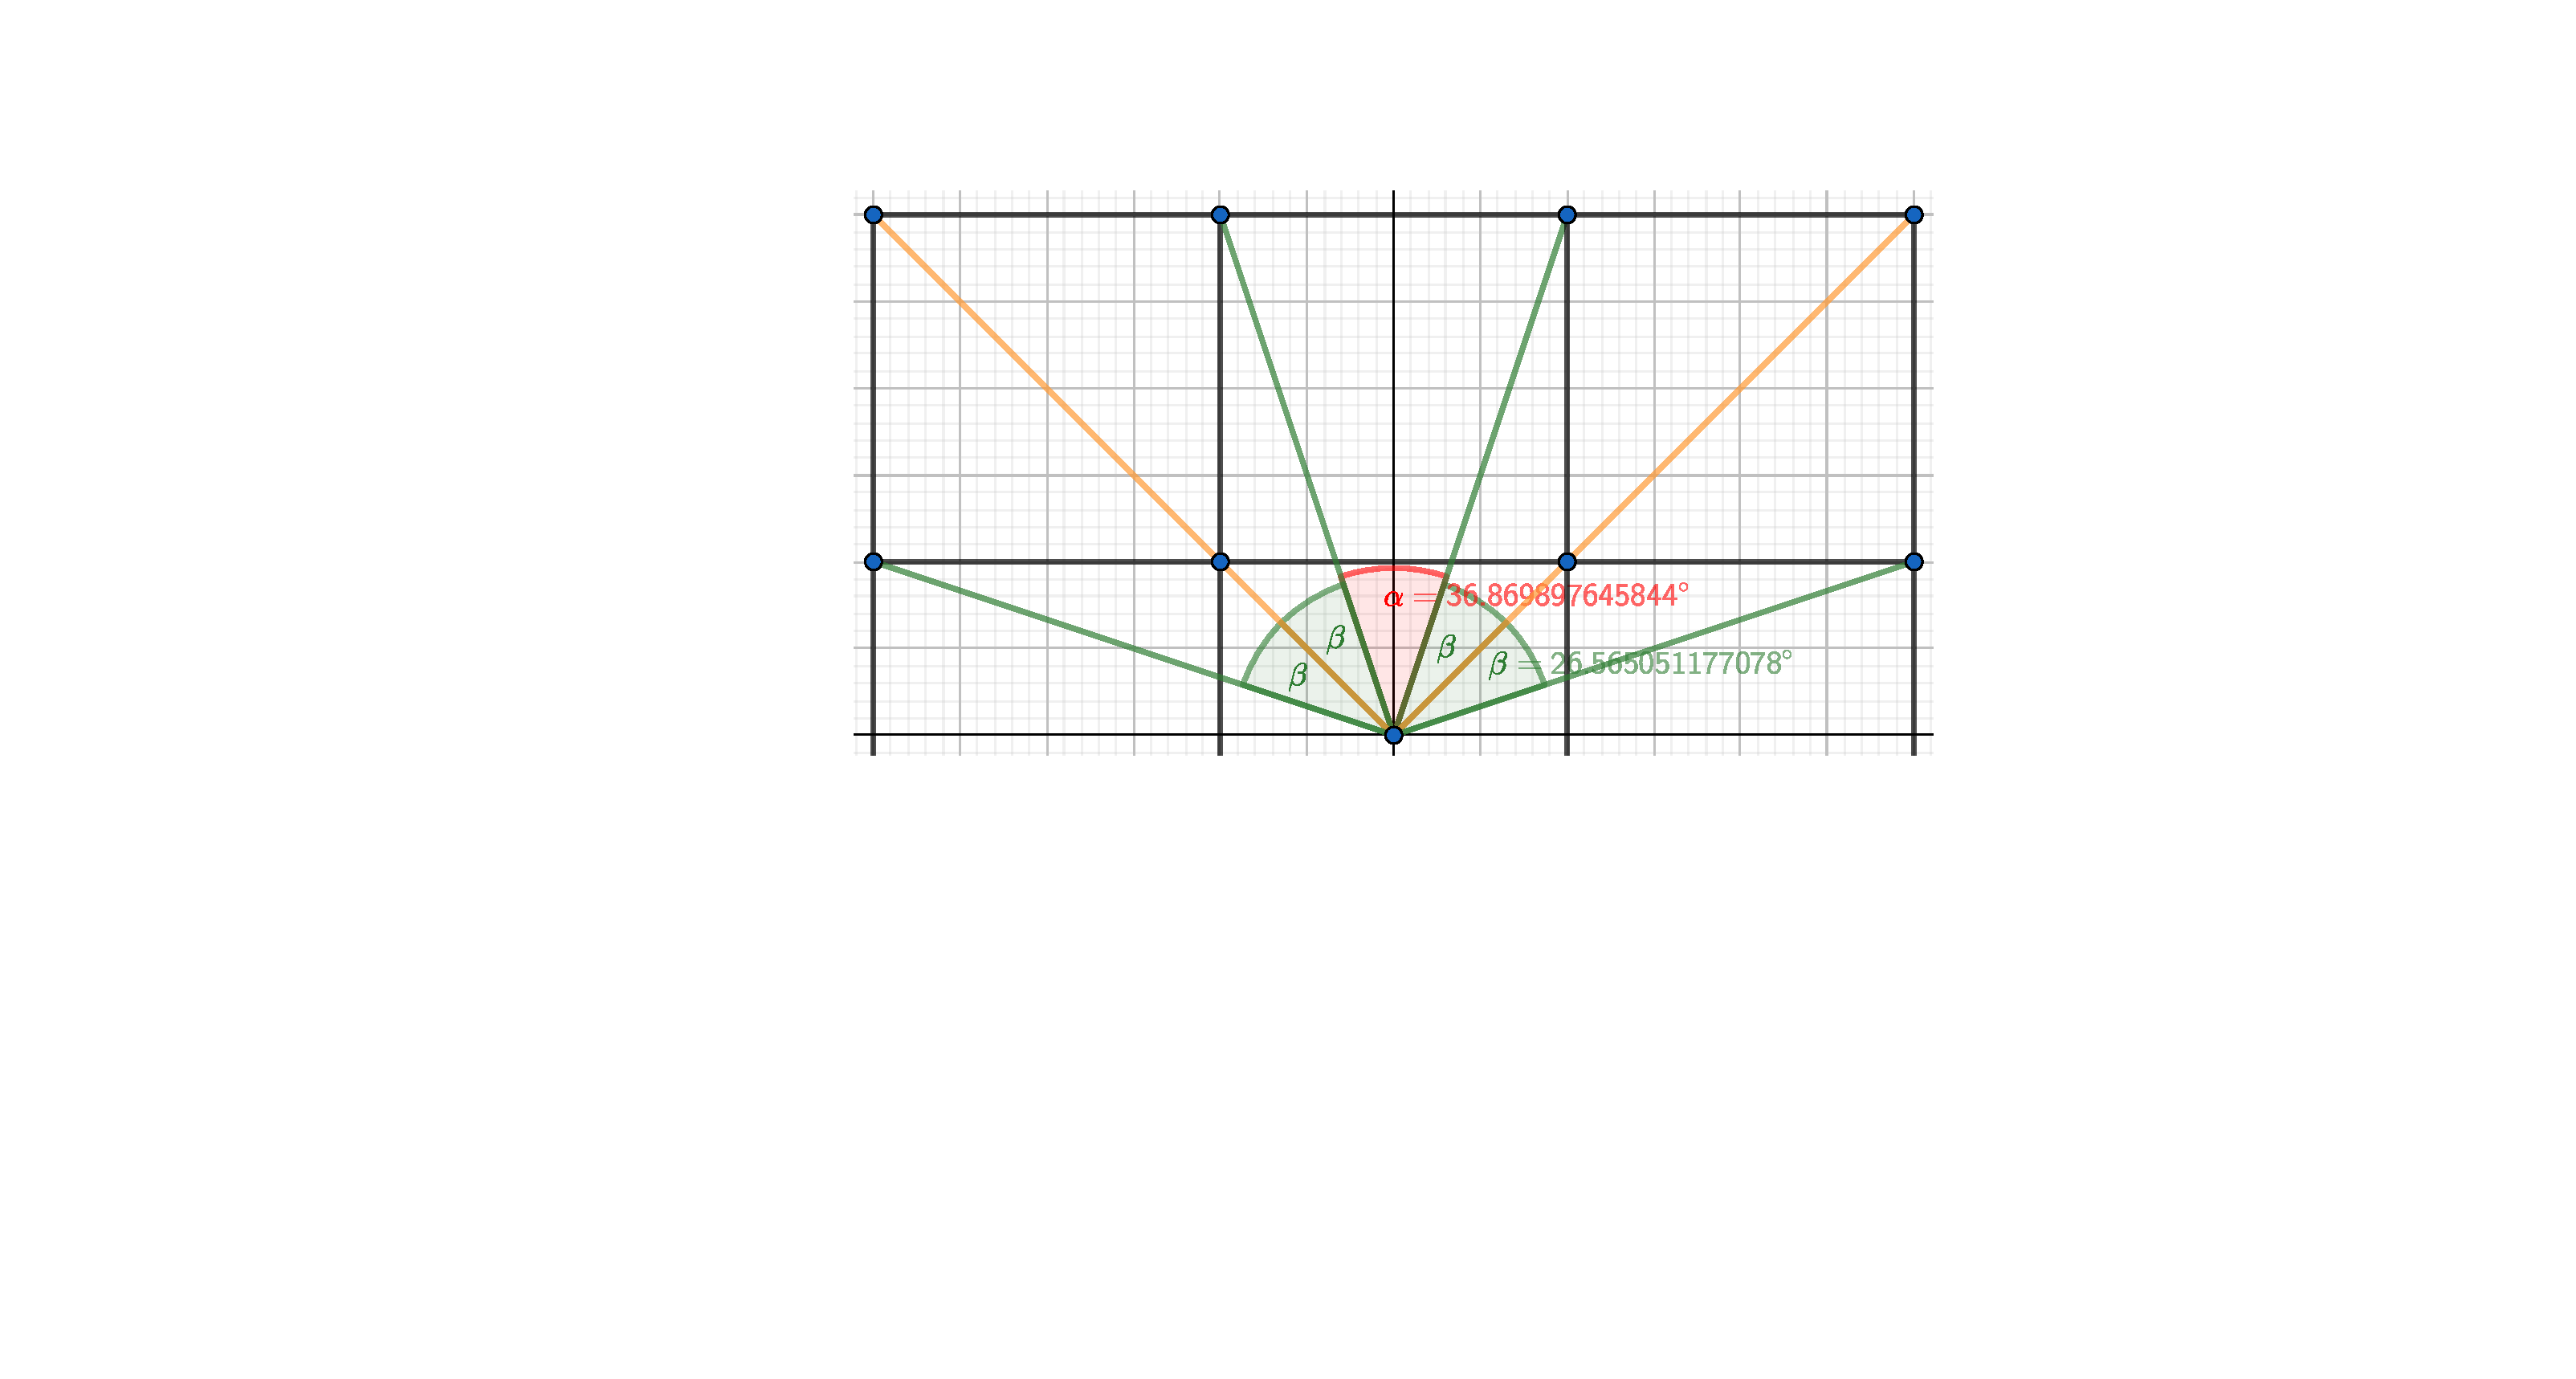
\includegraphics[width=\textwidth]
    {geogebra-export_large.pdf}
  }
  \caption{Propagation Scheme}
  \label{scheme}
\end{figure}

\end{column}
\end{columns}
} % END OF FRAME


\frame{
\frametitle{{Propagation Scheme}}
\begin{figure}[!t]
  \centering
 {
    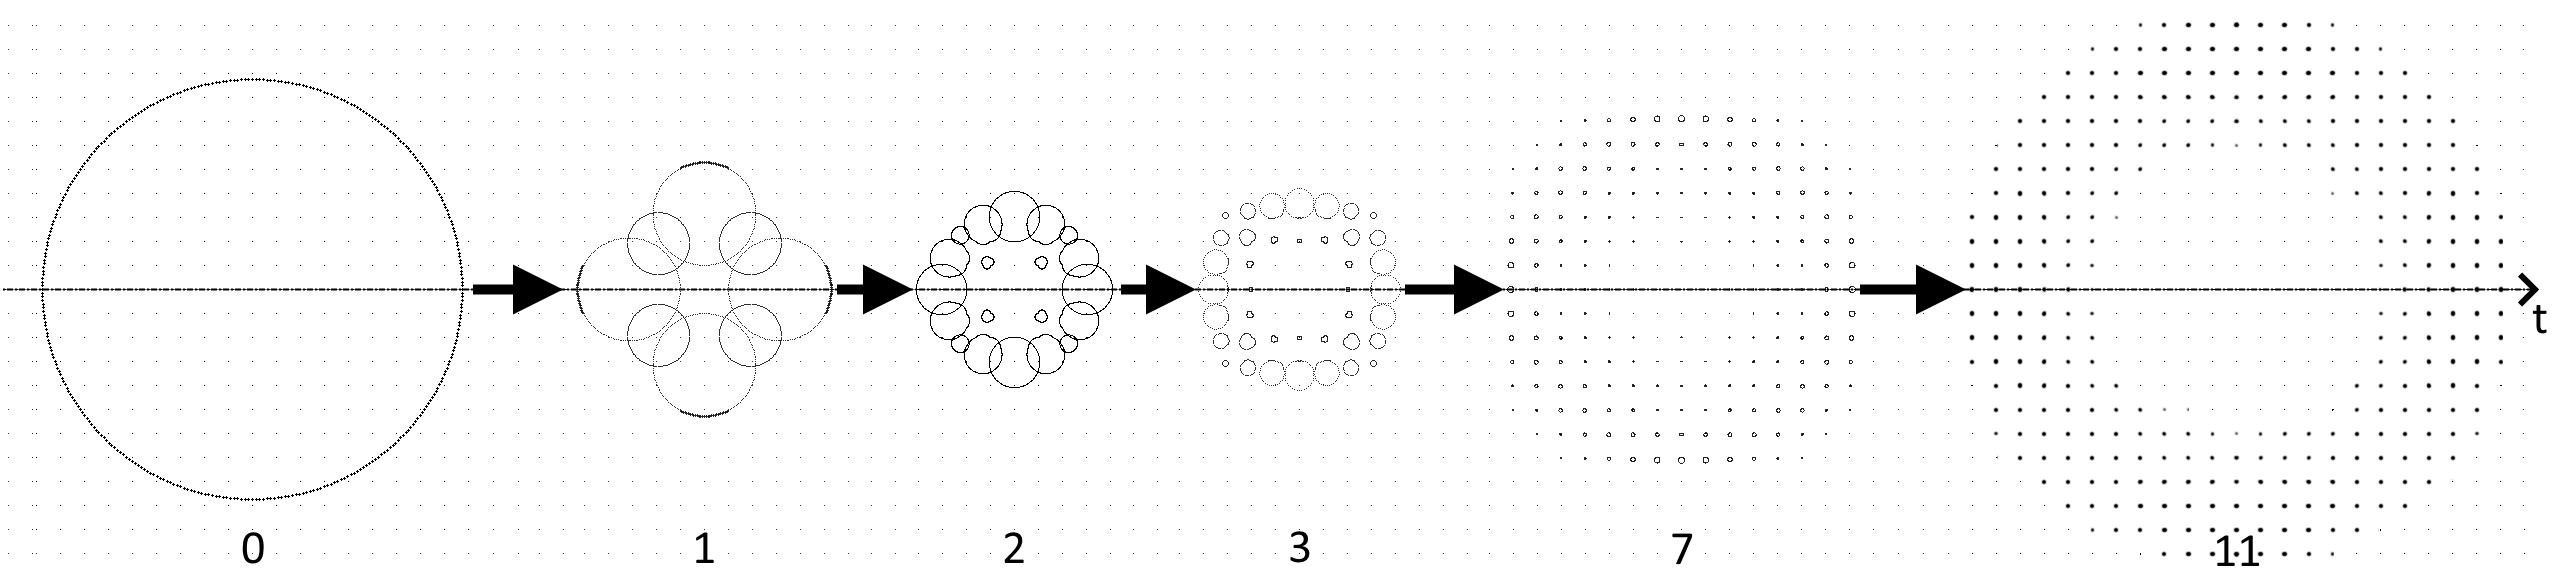
\includegraphics[width=0.8\textwidth]
    {steps_gallery_format_arrow_alt.png}
  }
  \caption{Impulse response}
  \label{scheme}
\end{figure}
\begin{align*}
\sum_{\cos_+} &= \int_{-\frac{\pi}{2}}^{\frac{\pi}{2}}\cos_+(\omega)\mathop{d\omega} \approx 2,\\
	\cos_k(\omega) &= \frac{\Phi_t}{\sum_{\cos_+}}cos_+(\omega-k\cdot\frac{\pi}{4})\hskip 20pt \mathit{with} \ k\in[0,7]
\end{align*}


} % END OF FRAME

\frame{
\frametitle{{Propagation Scheme - Procedure}}
\begin{block}{\centering \textbf{Steps}}

\begin{enumerate}
	\item Accumulation: Evaluating and Accumulating the Polar Profiles
	\item Applying the linear combination (partition) weights
	\item Injection: Scaling and Placing of a Cosine Lobe
\end{enumerate}
\end{block}\bigskip
For now, we are able to propagate intensities as circular waves in a 2D Cartesian grid defined through polar functions given on cell centers.
} % END OF FRAME

\frame{
\frametitle{{Transmission Profiles}}

\begin{block}{\centering \textbf{Ellipse Equation}}
\begin{align*}
	r(\omega) = \frac{ab}{\sqrt{a^{2}\sin^{2}(\omega-\varphi)+b^{2}\cos^{2}(\omega-\varphi)}} =\frac{\lambda_1\lambda_2}{\sqrt{\lambda_1^2\sin^2(\omega-\varphi)+\lambda_2^2\cos^2(\omega-\varphi)}}.
\end{align*}
\end{block}
\begin{itemize}
	\item transmission profiles $r(\omega)$ are given as symbolic functions by the mapping of eigenvalues to half-axes radii and the shift angle of the major eigenvector $\varphi=\mathop{atan2}\frac{s_{1,y}}{s_{1,x}}$ 
	\item these polar functions are precomputed and sampled once as an initialization step
\end{itemize}


} % END OF FRAME

\frame{
\frametitle{{Transmission Profiles}}
\begin{columns}
\begin{column}{.6\textwidth}
\begin{block}{\centering \textbf{Redefinition}}
\begin{align*}
	\Phi_{t} &= n_f\varepsilon_k\int T(\omega)I(\omega)\mathop{d\omega}\\
n_f &= \frac{\mean{T}\mean{I}}{\widebar{TI}}
\end{align*}
\end{block}
\begin{itemize}
	\item transmission profiles (cyan) are weighted with the intensity profiles (red) as a window function
	\item a normalization factor $n_f$ is required to respect energy conservation principles 
\end{itemize}

\end{column}

\begin{column}{.4\textwidth}
\begin{figure}[!t]
  \centering
 {
    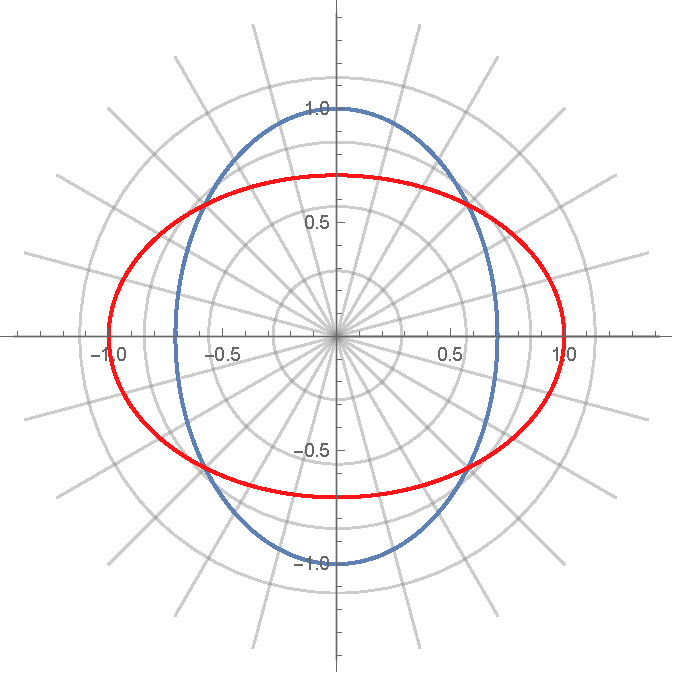
\includegraphics[width=0.6\textwidth]
    {polarplot.pdf}
  }
  \caption{Transmission Weighting}
  \label{scheme}
\end{figure}

\end{column}
\end{columns}
} % END OF FRAME

\frame{
\frametitle{{Propagation Scheme - Procedure}}
\begin{block}{\centering \textbf{Procedure}}

\begin{enumerate}
	\item Computation of normalization factor $n_f$
	\item Direction (component)-wise weighting to account for shared part in diagonal cones
	\item Integration (accumulation) of total radiant flux weighted with \underline{normalized} transmission profiles inside the angular neighbor range (read-access)
	\item Scaling of cosine lobe corresponding to neighbor direction and subsequent placing (injection) to corresponding neighbor (write-access)
\end{enumerate}
\begin{align*}
	\mathcal{C'} = \mathop{propagate}\{c_i\in \mathcal{C} \ \mid \ |\mean{I}_i| > 0\} \hskip 5pt {\forall } \ i \in [1,\mathop{dim}]
\end{align*}
\end{block}
Until now, we are able to modulate the propagated intensities with the anisotropy characteristics of the underlying tensor field.
} % END OF FRAME

\frame{
\frametitle{{Propagation Scheme}}
\begin{block}{\centering \textbf{Criterion}}
\begin{itemize}
	\item the Procedure is repeated recursively for each individual cell and is performed with switching source and target buffer
	\item a stop sequence is initiated when following criterion is reached:
	\begin{align*}
	\Delta \Phi_{total} &= \sum_{c_i\in\mathcal{C}}\lvert\Delta I_i(\omega)\rvert = \sum_{c_i\in\mathcal{C}} \int_0^{2\pi} \lvert(I'_i(\omega)-I_i(\omega))\rvert \mathop{d\omega}  \overset{!}{<} \epsilon.
	\end{align*}
	\item we gather the total energy in the field and compare it to the last iteration until a state of equilibrium is reached, whereas the flow map t in a stable state
\end{itemize}
\end{block}
} % END OF FRAME

\frame{
\frametitle{{Propagation Scheme - Physical Model}}
\begin{block}{\centering \textbf{Crystal Fiber Structures}}
\begin{itemize}
	\item crystal lattices reveal gradients in refractive indices, which lead to anisotropic light transport inside the medium (birefringence)
	\item the propability for redistribution of a photon in a particular direction is given by the phase function model yielded from Rayleigh scattering:
	\begin{align*}
 	P(\omega) &= \frac{T(\omega)}{\int_{k\pi}^{(k+1)\pi}T(\omega)\mathop{d\omega}}\\
 	\mathit{with} \int_0^{\pi} P(\omega) &= 1.
	\end{align*}
	\item each tensor is then a unique footprint: $\mathbf{t_{i,j}}\mapsto T(\omega)$
\end{itemize}
\end{block}
} % END OF FRAME

\frame{
\frametitle{{Propagation Scheme - Light Distributions}}
\begin{figure}[!t]
\centering
   a)
  \begin{minipage}{0.25\textwidth}
  \centering
    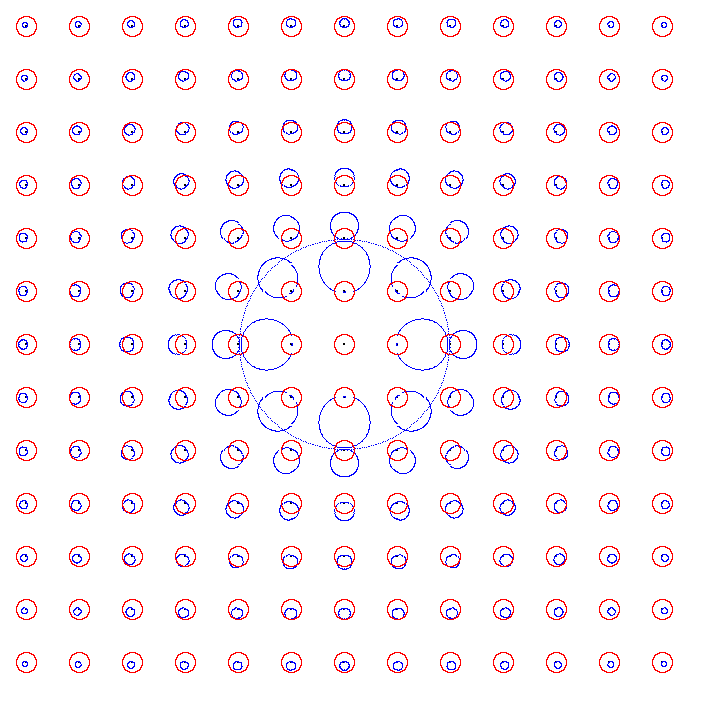
\includegraphics[width=0.7\textwidth]{isotropic-all-center.png}
    \label{a)}
  \end{minipage}
  \begin{minipage}{0.25\textwidth}
  \centering
    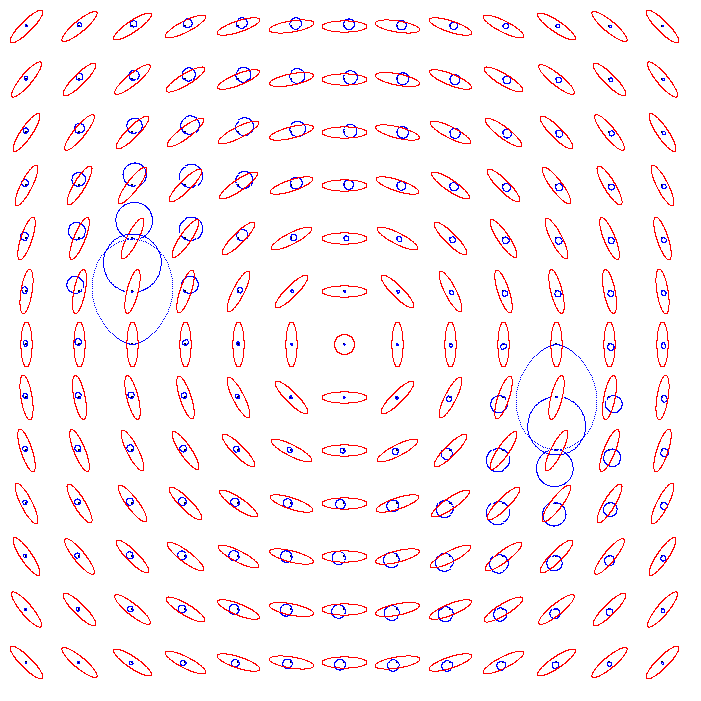
\includegraphics[width=0.7\textwidth]{rings-two-special1.png}
    \label{b)}
  \end{minipage}
  \begin{minipage}{0.25\textwidth}
    \centering
    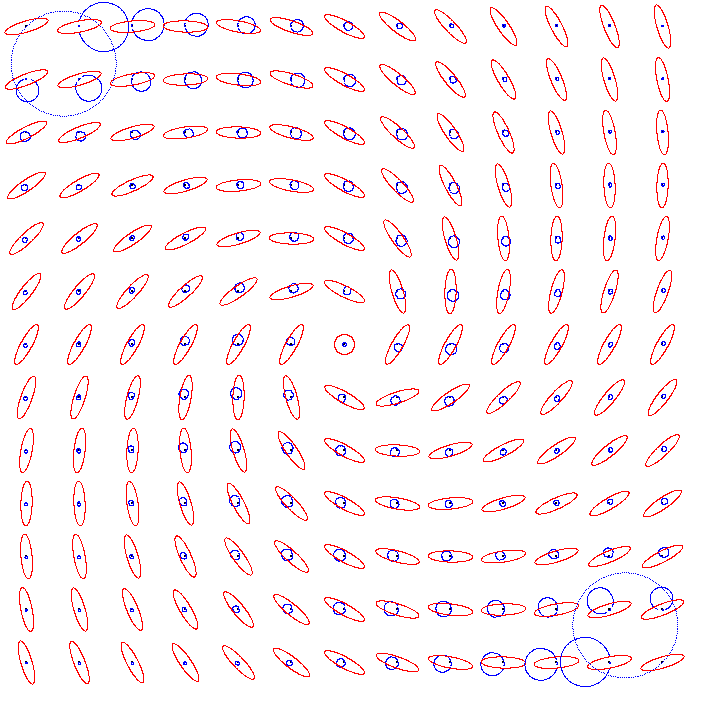
\includegraphics[width=0.7\textwidth]{spiral-two-wide.png}
    \label{b)}
  \end{minipage}
\label{isotropic}
\end{figure}
\begin{figure}[!t]
\centering
   b)
  \begin{minipage}{0.25\textwidth}
    \centering
    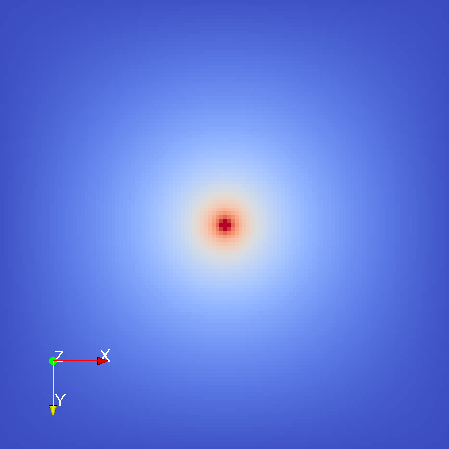
\includegraphics[width=0.7\textwidth]{iso_sat.png}
    \label{a)}
  \end{minipage}
  \begin{minipage}{0.25\textwidth}
    \centering
    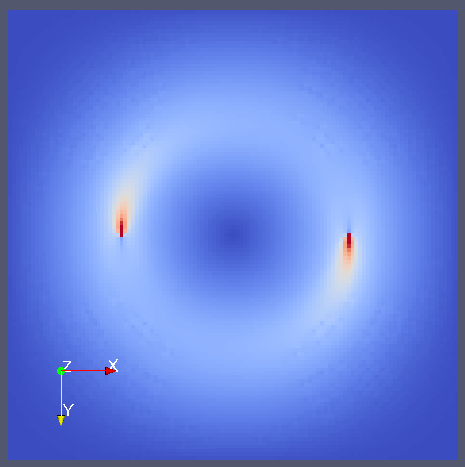
\includegraphics[width=0.7\textwidth]{cos_parallel.png}
    \label{b)}
  \end{minipage}
  \begin{minipage}{0.25\textwidth}
    \centering
    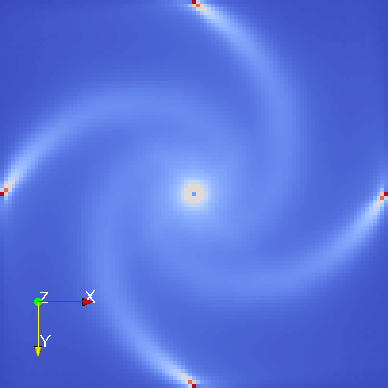
\includegraphics[width=0.7\textwidth]{spiral_full.png}
    \label{b)}
  \end{minipage}
\caption{final light propagation distributions in: a) polar, b) scalar field rep}
\label{rings-tests}
\end{figure}

} % END OF FRAME

\frame{
\frametitle{{Light Transport Gradient - Evolution}}
\begin{figure}[!t]
\centering
 a)
  \begin{minipage}{0.25\textwidth}
    \centering
    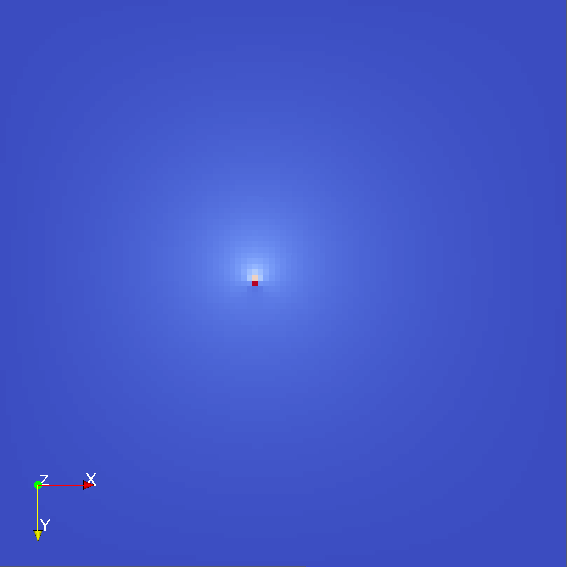
\includegraphics[height=0.7\textwidth]{scalar_iso_left.png}
    \label{a)}
  \end{minipage} $-$
  \begin{minipage}{0.25\textwidth}
    \centering
    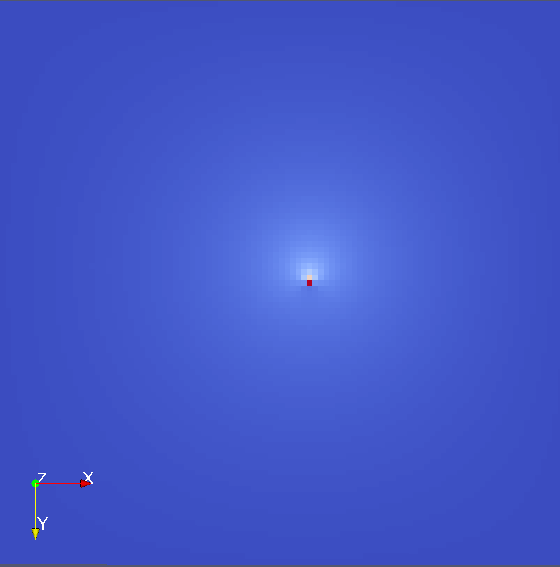
\includegraphics[height=0.7\textwidth]{scalar_iso_right.png}
    \label{b)}
  \end{minipage} $=$
   \begin{minipage}{0.25\textwidth}
    \centering
    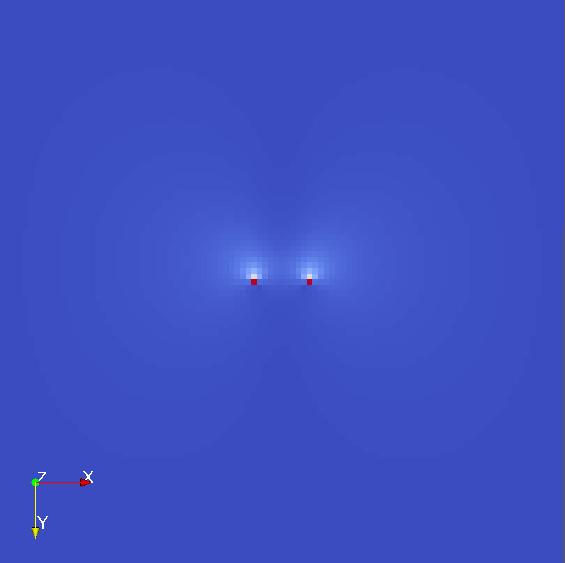
\includegraphics[height=0.7\textwidth]{scalar_iso_diff.png}
    \label{b)}
  \end{minipage}
\label{analysis1}
\end{figure}
\begin{figure}[!t]
\centering
 b)
  \begin{minipage}{0.25\textwidth}
    \centering
    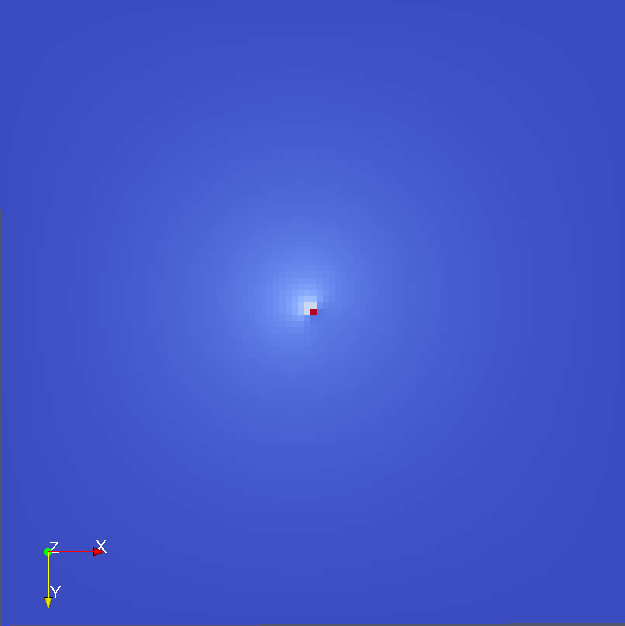
\includegraphics[height=0.7\textwidth]{scalar_iso_leftangle.png}
    \label{a)}
  \end{minipage} $-$
  \begin{minipage}{0.25\textwidth}
    \centering
    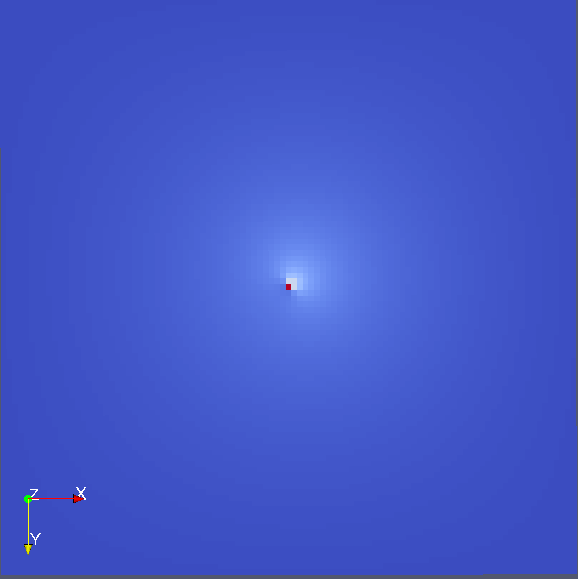
\includegraphics[height=0.7\textwidth]{scalar_iso_rightangle.png}
    \label{b)}
	\end{minipage} $=$
   \begin{minipage}{0.25\textwidth}
    \centering
    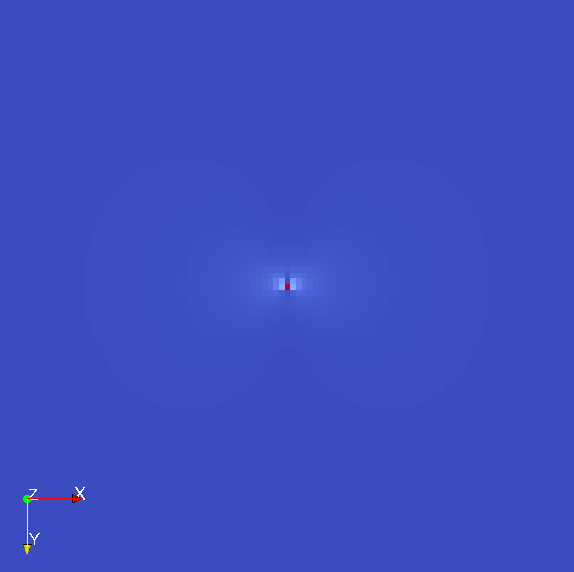
\includegraphics[height=0.7\textwidth]{scalar_iso_anglediff.png}
    \label{b)}
  \end{minipage}
  \caption{Isotropic test field}
\label{analysis2}
\end{figure}

} % END OF FRAME

\frame{
\frametitle{{Light Transport Gradient - Evolution}}
\begin{figure}[!t]
\centering
 a)
  \begin{minipage}{0.25\textwidth}
    \centering
    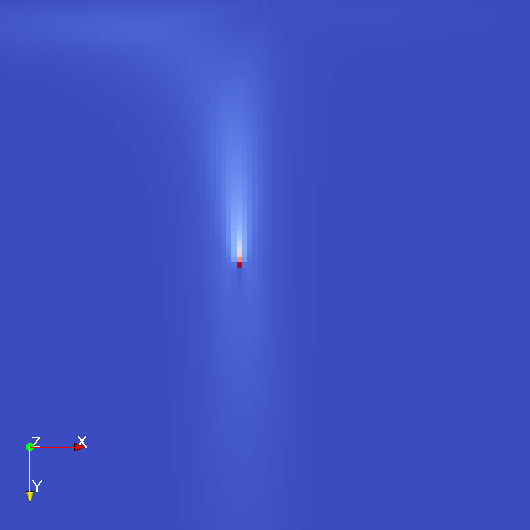
\includegraphics[height=0.7\textwidth]{ftle_left.png}
    \label{a)}
  \end{minipage} $-$
  \begin{minipage}{0.25\textwidth}
    \centering
    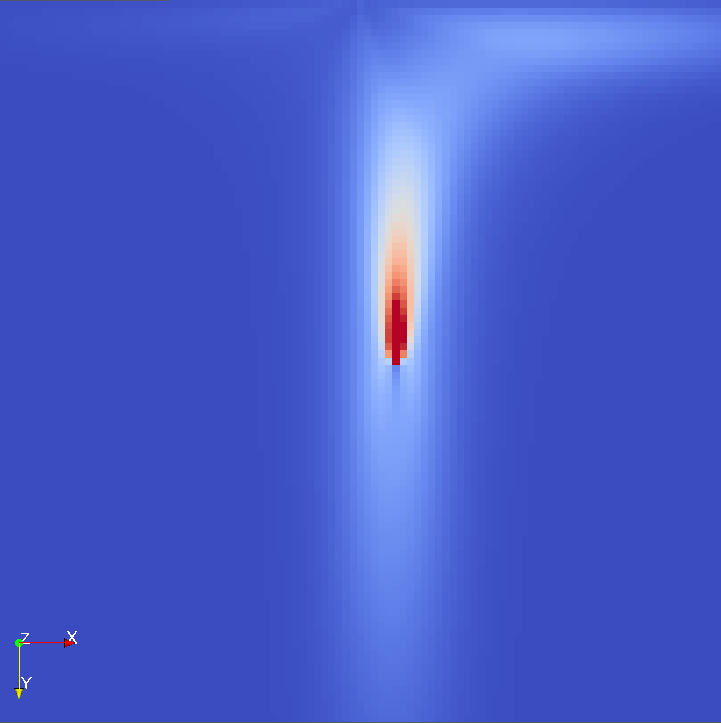
\includegraphics[height=0.7\textwidth]{ftle_right.png}
    \label{b)}
  \end{minipage} $=$
   \begin{minipage}{0.25\textwidth}
    \centering
    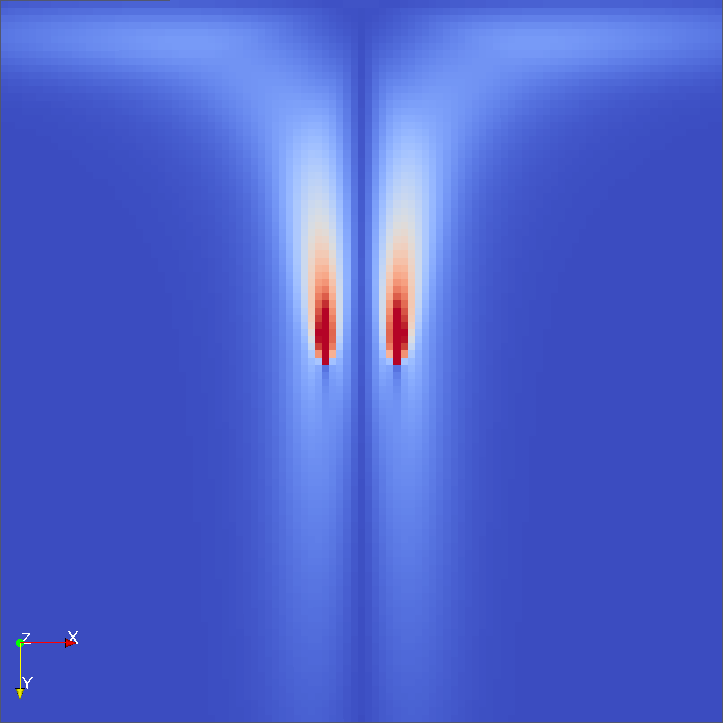
\includegraphics[height=0.7\textwidth]{ftle_diff.png}
    \label{b)}
  \end{minipage}
\label{analysis1}
\end{figure}
\begin{figure}[!t]
\centering
 b)
  \begin{minipage}{0.25\textwidth}
    \centering
    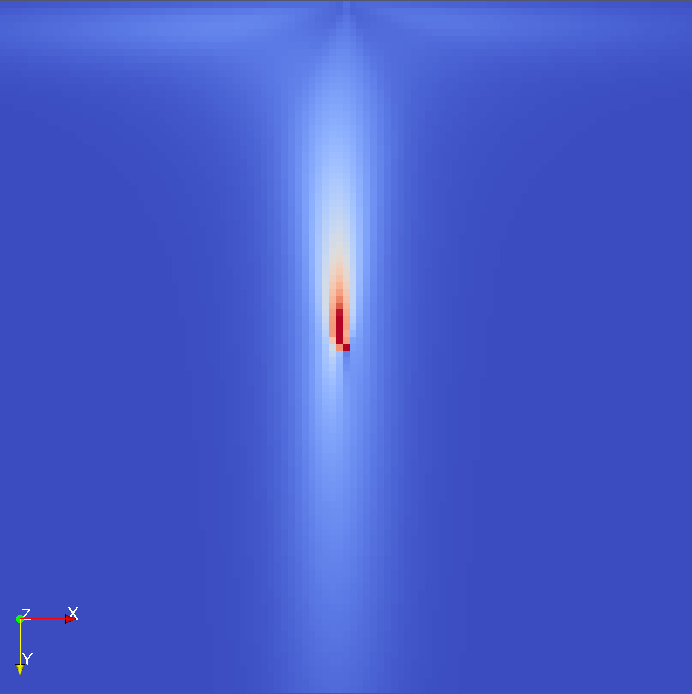
\includegraphics[height=0.7\textwidth]{ftle_leftangle.png}
    \label{a)}
  \end{minipage} $-$
  \begin{minipage}{0.25\textwidth}
    \centering
    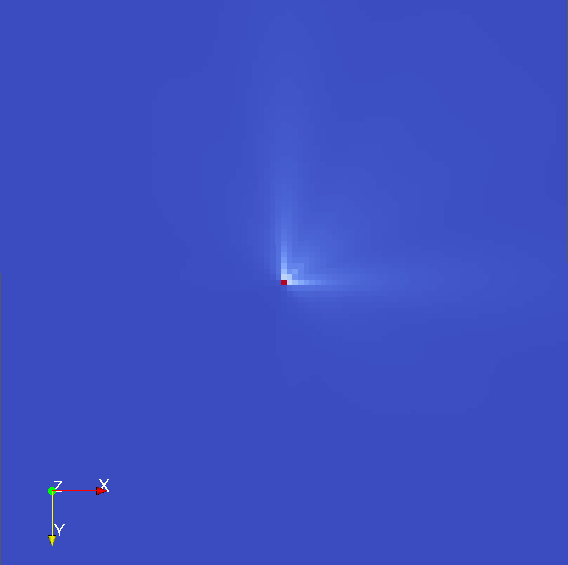
\includegraphics[height=0.7\textwidth]{ftle_rightangle.png}
    \label{b)}
	\end{minipage} $=$
   \begin{minipage}{0.25\textwidth}
    \centering
    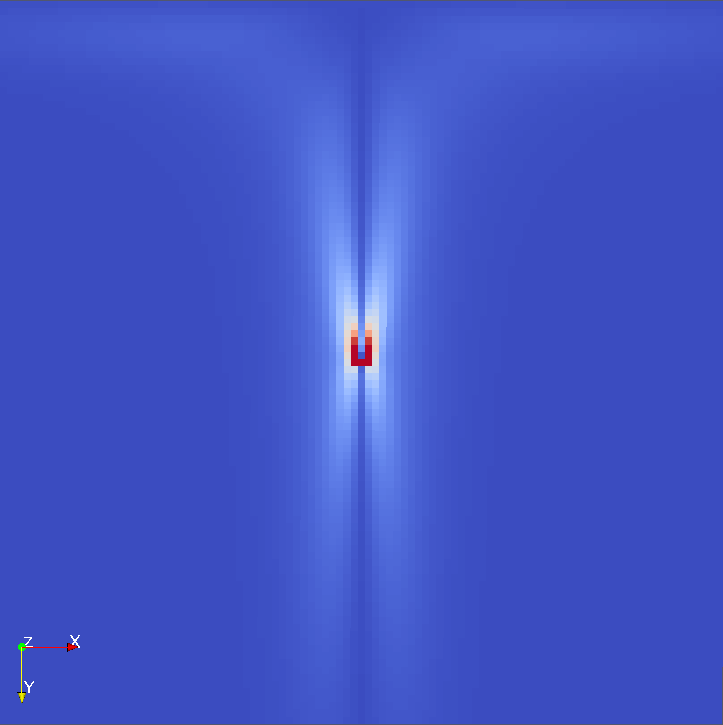
\includegraphics[height=0.7\textwidth]{ftle_anglediff.png}
    \label{b)}
  \end{minipage}
  \caption{Drain test field}
\label{analysis2}
\end{figure}

} % END OF FRAME

\frame{
\frametitle{{Light Transport Gradient - Definition}}
\begin{block}{\centering \textbf{Defintion}}
\begin{align*}
	\mathcal{B} = \mathop{propagate}\{c_i\in \mathcal{C} \ \mid \ |\mean{I}_i| > 0\} \ {\forall } \ i \in [1,\mathop{dim}] \ {\forall } \ j \in [1,\mathop{dim}\cdot \mathop{steps}]
	\label{ftle}
\end{align*}
\end{block}
\begin{itemize}
	\item Previous examples prove that the conductivity property (transmission) of the tensor field effects a separation of energies for diverging pathlines
	\item the eventual goal is to obtain a FTLE field from accumulating the overall energy in the difference scalar field
	\item Buffer $\mathcal{B} = \{\mathcal{C}_1, \mathcal{C}_2, ..., \mathcal{C}_j\}$ contains propagated light distributions for each discrete location and direction in the field, on which we will eventually apply a gradient
\end{itemize}
} % END OF FRAME

\frame{
\frametitle{{Light Transport Gradient - Definition}}
\begin{block}{\centering \textbf{Gradient Approximation: Central Differences}}
\begin{align*}
	\nabla \mathbf{b}_{x,y,\omega} =
	\begin{pmatrix}
	\frac{\partial \mathbf{b}_{x,y,\omega}}{\partial x} \\ \frac{\partial \mathbf{b}_{x,y,\omega}}{\partial y} \\ \frac{\partial \mathbf{b}_{x,y,\omega}}{\partial \omega}
	\end{pmatrix} \approx
	\frac{1}{2}
	\begin{pmatrix}
	\sum_{\mathbf{c}}\lvert \mathbf{b}_{x+1,y,\omega} - \mathbf{b}_{x-1,y,\omega}\rvert \\ \sum_{\mathbf{c}}\lvert \mathbf{b}_{x,y+1,\omega} - \mathbf{b}_{x,y-1,\omega}\rvert \\ \sum_{\mathbf{c}}\lvert \mathbf{b}_{x,y,\omega+\pi/6} - \mathbf{b}_{x,y,\omega-\pi/6}\rvert
	\end{pmatrix} =
	\frac{1}{2}
	\begin{pmatrix}
	\sum_{\mathbf{c}\in \mathbf{b_x}}\lvert \mathbf{b_x}\rvert \\ \sum_{\mathbf{c}\in \mathbf{b_y}}\lvert\mathbf{b_{y}}\rvert \\ \sum_{\mathbf{c}\in \mathbf{b_{\omega}}}\lvert \mathbf{b_{\omega}}\rvert
	\end{pmatrix}.
\end{align*}
\end{block}
\begin{itemize}
	\item a finite set of cells is interpreted as a 1D vector $\mathcal{C}_{final}=\mathbf{b}\in\mathcal{B}$ here, contained as an element of the set of final buffers $\mathcal{B}$
	\item the resulting volume grid is raised by one dimension $d=2+1=3$ for taking direction as additional input parameter and computing the Euclidean norm of the gradient
	
\end{itemize}
} % END OF FRAME

%\item runtime behavior: $T(n)=\mathcal{O}(\mathop{width}\mathop{width}\mathop{steps}\mathop{width}\mathop{width}\mathop{steps}\mathop{width}) = \mathcal{O}(\mathop{width^5}\mathop{steps^2})$


\frame{
\frametitle{{Light Transport Gradient - Functionality}}
\begin{columns}
\begin{column}{.5\textwidth}
\begin{itemize}
	\item Isotropic test field reveals offset response for the approach
	\bigskip
	\item Natural shift against the inital light source (slice) direction (left)
	\bigskip
	\item maximum distance to the edges lies on the circumference of a circle
\end{itemize}
\end{column}
\begin{column}{.5\textwidth}
\begin{figure}[t]

\includegraphics[width=0.4\textwidth]{isotropic2.png} a)
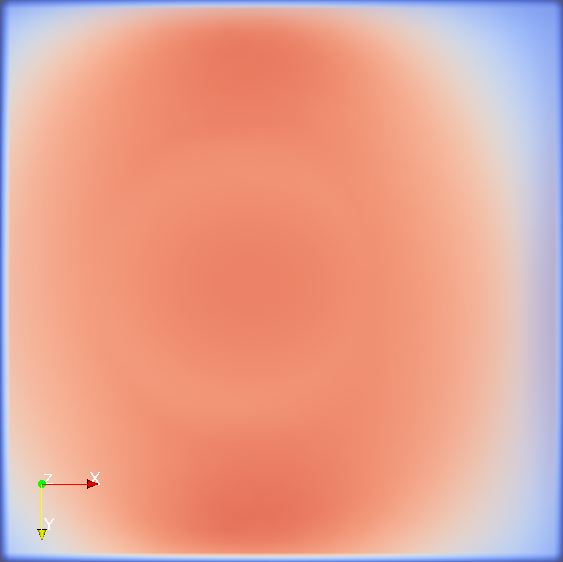
\includegraphics[width=0.4\textwidth]{iso_ftle.png} b)
\caption{Isotropic test field: a) Glyphs, b) LTG}
\end{figure}

\end{column}
\end{columns}

} % END OF FRAME

\frame{
\frametitle{{Light Transport Gradient - Isotropic field}}
\begin{columns}
\begin{column}{.5\textwidth}
\begin{itemize}
	\item Isotropic test field reveals offset response for the approach
	\bigskip
	\item Natural shift against the inital light source (slice) direction (left)
	\bigskip
	\item maximum distance to the edges lies on the circumference of a circle
\end{itemize}
\end{column}
\begin{column}{.5\textwidth}
\begin{figure}[t]
\includegraphics[height=0.5\textwidth]{iso_volume.png} a)
\includegraphics[height=0.5\textwidth]{iso_isovolume.png} b)
\caption{Isotropic test field: a) Glyphs, b) LTG}
\end{figure}

\end{column}
\end{columns}

} % END OF FRAME

\frame{
\frametitle{{Light Transport Gradient - Drain field}}
\begin{figure}[!t]
\centering
  \begin{minipage}{0.3\textwidth}
	\centering
    \includegraphics[width=0.8\textwidth]{drain(alt)-TFL.png}
    \label{a)}
	a)~TFLs and glyphs
  \end{minipage}
  \begin{minipage}{0.3\textwidth}
  \centering
    \includegraphics[width=0.8\textwidth]{ftle_drain_alt.png}
    \label{b)}
	b)~LTG($90^\circ$) for a)
  \end{minipage}
  \begin{minipage}{0.3\textwidth}
  \centering
    \includegraphics[width=0.8\textwidth]{drain_alt_gradient.png}
    \label{b)}
	c)~Gradient for b)
  \end{minipage}
  \caption{Drain test field}
\label{ftle_base}
\end{figure}
\begin{itemize}
	\item strong ridge in the center of the field indicated by the approach
	\item segmentation could be done by edge detection via gradient filter
\end{itemize}
} % END OF FRAME

\frame{
\frametitle{{Light Transport Gradient - Drain field}}
\begin{columns}
\begin{column}{.5\textwidth}
\begin{itemize}
	\item Drain test field reveals strong ridge in $-y$ direction
	\bigskip
	\item Ridge remains more stable on the top edges w.r.t. initial direction
\end{itemize}
\end{column}
\begin{column}{.5\textwidth}
\begin{figure}[!t]
\centering
  \begin{minipage}{0.4\textwidth}
  \includegraphics[width=0.9\textwidth]{drain_top.PNG}\vskip 10pt
    \includegraphics[width=0.9\textwidth]{drain_alt-profile.PNG}
	a)
    \label{a)}
  \end{minipage}
  \begin{minipage}{0.4\textwidth}
    \includegraphics[width=0.9\textwidth]{drain_alt_isovolume.PNG}
	b)
    \label{b)}
  \end{minipage}
  \caption{LTG volumes: Drain test field a) cross-section, b) IsoVolume}
\label{drain_contour}
\end{figure}

\end{column}
\end{columns}

} % END OF FRAME

\frame{
\frametitle{{Light Transport Gradient - Inverse field}}
\begin{columns}
\begin{column}{.5\textwidth}
\begin{itemize}
	\item Inverse test field reveals strong ridges in axes direction
	\bigskip
	\item Ridges are detected up to orthogonally to the initial light source direction
\end{itemize}
\end{column}
\begin{column}{.5\textwidth}
\begin{figure}[!t]
\centering
  \begin{minipage}{0.4\textwidth}
  \centering
    \includegraphics[width=0.9\textwidth]{inverse-TFL.png}
    \label{a)}
	a)
  \end{minipage}
  \begin{minipage}[!t]{0.4\textwidth}
  \centering
    \includegraphics[width=0.9\textwidth]{inverse-FTLE-raw.png}
    \label{b)}
	b)
  \end{minipage}
  \caption{Inverse-test field: a) TFLs and glyphs, b) LTG($90^\circ$) for a)}
\label{inverse-ftle}
\end{figure}
\end{column}
\end{columns}

} % END OF FRAME

\frame{
\frametitle{{Light Transport Gradient - Inverse field}}
\begin{figure}[!t]
\centering
  \begin{minipage}{0.3\textwidth}
    \includegraphics[height=0.7\textwidth]{inverse_isovolume.png}
    a)
  \end{minipage}
  \begin{minipage}{0.3\textwidth}
    \includegraphics[height=0.7\textwidth]{inverse_surface.png}
    b)
  \end{minipage}
   \begin{minipage}{0.3\textwidth}
    \includegraphics[height=0.7\textwidth]{inverse_contour.png}
    c)
  \end{minipage}
    \caption{LTG volumes: ``Inverse'' test field: a) IsoVolume, b) Surface, c) Contour}
\label{inverse_volume}
\end{figure}
\begin{itemize}
	\item Inverse test field reveals strong ridges in axes direction
	\item Ridges are detected up to orthogonally to the initial light source direction
\end{itemize}
} % END OF FRAME

%\frame{
%\frametitle{{Light Transport Gradient - Functionality}}
%\begin{figure}[!t]
%\centering
%  \begin{minipage}{0.4\textwidth}
%  \centering
%    \includegraphics[width=0.9\textwidth]{bow-TFL.png}
%    \label{a)}
%	a)
%  \end{minipage}
%  \begin{minipage}[!t]{0.4\textwidth}
%  \centering
%    \includegraphics[width=0.9\textwidth]{bow_ftle.png}
%    \label{b)}
%	b)
%  \end{minipage}
%  \caption{``Bow''-test field: a) TFLs and glyphs, b) LTG($0^\circ$) for a)}
%\label{bow-ftle}
%\end{figure}
%
%} % END OF FRAME
%
%\frame{
%\frametitle{{Light Transport Gradient - Functionality}}
%\begin{figure}[!t]
%\centering
%  \begin{minipage}{0.4\textwidth}
%  \centering
%    \includegraphics[width=\textwidth]{bow_contour.png}
%	a)
%  \end{minipage}
%  \begin{minipage}{0.4\textwidth}
%  \centering
%    \includegraphics[width=\textwidth]{bow_volume.png}
%	b)
%  \end{minipage}
%    \caption{LTG volumes: ``Bow'' test field : a) Contour, b) IsoVolume}
%\label{bow_contour}
%\end{figure}
%
%} % END OF FRAME


\section[Results and Evaluation]{Results and Evaluation}
%----------------------------------------


\frame{
\frametitle{{Evaluation - Inverse Law}}
\begin{columns}
\begin{column}{.5\textwidth}
\begin{itemize}
	\item Inverse (square) law is evaluated for propagation
	\bigskip
	\item Magnitude is related to magnitude $r_1$ at distance 1 
	\bigskip
	\item Samples are fitted to $f(r)=\frac{a}{r}+c$
\end{itemize}
\end{column}
\begin{column}{.5\textwidth}
\begin{figure}[!t]
  \centering
 {
    \includegraphics[width=0.6\textwidth]
    {inverse_law.pdf}
  }
  \caption{Propagation attenuation}
  \label{att}
\end{figure}

\end{column}
\end{columns}

} % END OF FRAME

\frame{
\frametitle{{Evaluation - Total Anisotropy}}
\begin{figure}[!t]
\centering
  \begin{minipage}{0.3\textwidth}
  \centering
    \includegraphics[width=0.8\textwidth]{tensorfieldlines.png}
	a) TFLs and glyphs
    \label{a)}
  \end{minipage}
  \begin{minipage}{0.3\textwidth}
  \centering
    \includegraphics[width=0.8\textwidth]{total_anisotropy1.png}
    b) iteration $50$
    \label{b)}
  \end{minipage}
  \begin{minipage}{0.3\textwidth}
  \centering
    \includegraphics[width=0.8\textwidth]{total_anisotropy2.png}
	c) iteration $103$
    \label{c)}
  \end{minipage}
\caption{intensity propagation in grid for total anisotropy}
\label{anisotropy}
\end{figure}
Light intensity is propagated in circular orbits, which reveals a sampling drift.
} % END OF FRAME

\frame{
\frametitle{{Evaluation - Light Transport Gradient}}
\begin{figure}[!t]
\centering
  \begin{minipage}[t]{0.3\textwidth}
    \centering
  \includegraphics[height=0.7\textwidth]{gyre.png}
	a)
    \label{a)}
  \end{minipage}
  \begin{minipage}[t]{0.3\textwidth}
    \centering
    \includegraphics[height=0.7\textwidth]{gyre_ftle.PNG}
	b)
    \label{b)}
  \end{minipage}
  \begin{minipage}[t]{0.3\textwidth}
    \centering
    \includegraphics[height=0.7\textwidth]{gyre_ftle_org.PNG}
	c)
    \label{b)}
  \end{minipage}
  \caption{Gyre test field: a) glyphs, b) LTG($0^\circ$), c) FTLE: Hlawatsch's approach}
\label{gyre-ftle}
\end{figure}
\begin{itemize}
	\item LTG is detecting ridges up to orthogonal directions
	\item Response is decreased in gyre centers for measuring separation through (circular) overlap
\end{itemize}
} % END OF FRAME

\frame{
\frametitle{{Evaluation - Light Transport Gradient}}
\begin{figure}[!t]
\centering
  \begin{minipage}{0.3\textwidth}
    \centering
  \includegraphics[height=0.7\textwidth]{gyre_volume2.png}
	a)
    \label{a)}
  \end{minipage}
  \begin{minipage}{0.3\textwidth}
    \centering
    \includegraphics[height=0.7\textwidth]{gyre_gauss_contour.PNG}
	b)
    \label{b)}
  \end{minipage}
   \begin{minipage}{0.3\textwidth}
     \centering
    \includegraphics[height=0.7\textwidth]{gyre_volume4.PNG}
	c)
    \label{b)}
  \end{minipage}
  \caption{Gyre test field LTG volumes: a) IsoVolume, b) Contour, c) GaussContour}
\label{gyre_volume}
\end{figure}

\begin{itemize}
	\item LTG is detecting ridges up to orthogonal directions
	\item Response is decreased in gyre centers for measuring separation through (circular) overlap
\end{itemize}
} % END OF FRAME


\frame{
\frametitle{{Evaluation - Light Transport Gradient}}
\begin{itemize}
	\item real data examples reveal two important features, which need to be respected: 
	\begin{enumerate}
		\item  Segmentation in FG-BG regions
		\item Random noise modulated on top
	\end{enumerate}
	\item We propose the following threshold corrections to prevent noisy FTLE results: 
	\begin{itemize}
		\item for Hlawatsch's approach:
			\begin{align*}
		\varphi_i = 
		\begin{cases}
	    	\varphi_i,& \text{if } \mean{r}_i > \theta,\\
 	   		0.0^\circ,              & \text{otherwise}.
		\end{cases}
			\end{align*}
		\item for our approach (only for transmission - extending trajectories):
		\begin{align*}
		r_i(\omega) = 
		\begin{cases}
	    	\frac{1}{\mean{r}_i}r_i(\omega),& \text{if } \mean{r}_i > \theta,\\
 	   		1.0,              & \text{otherwise}.
		\end{cases}
		\end{align*}
	\end{itemize}

\end{itemize}
} % END OF FRAME

\frame{
\frametitle{{Light Transport Gradient - Brain dataset}}
\begin{figure}[!t]
\centering
  \begin{minipage}{0.3\textwidth}
   \centering
  \includegraphics[height=0.7\textwidth]{brainDwnsmpl.png}
	a)~Glyphs
    \label{a)}
  \end{minipage}
  \begin{minipage}{0.3\textwidth}
   \centering
    \includegraphics[height=0.7\textwidth]{brainDwnsmpl-TFL.PNG}
	b)~TFLs
    \label{b)}
  \end{minipage}
  \begin{minipage}{0.3\textwidth}
   \centering
    \includegraphics[height=0.7\textwidth]{brain_ftle_org.PNG}
	c)~FTLE: H.'s approach
    \label{b)}
  \end{minipage}
\caption{Brain test field}
\label{brain_ftle_comp}
\end{figure}

\begin{itemize}
	\item Noise present in the Brain dataset $\Rightarrow$ TFLs reveal chaotic trajectories
	\item FTLE response throughout the image (because of ambiguity in isotropic regions)
\end{itemize}
} % END OF FRAME

\frame{
\frametitle{{Light Transport Gradient - Brain dataset}}
\begin{figure}[!t]
\centering
  \begin{minipage}{0.3\textwidth}
   \centering
  \includegraphics[height=0.7\textwidth]{brainDwnsmpl_denoise.png}
	a)~Glyphs
    \label{a)}
  \end{minipage}
  \begin{minipage}{0.3\textwidth}
   \centering
    \includegraphics[height=0.7\textwidth]{brain-TFL.PNG}
	b)~TFLs
    \label{b)}
  \end{minipage}
  \begin{minipage}{0.3\textwidth}
   \centering
    \includegraphics[height=0.7\textwidth]{brain_ftle_surf_noisereduction.PNG}
	c)~FTLE: H.'s approach
    \label{b)}
  \end{minipage}
\caption{Brain test field (denoised)}
\label{brain_ftle_comp}
\end{figure}

\begin{itemize}
	\item Denoising: Tensor mags. below threshold are padded with zeros
	\item Correlating trajectories in BG regions: FTLE response only in FG regions
\end{itemize}
} % END OF FRAME

\frame{
\frametitle{{Light Transport Gradient - Brain dataset}}
\begin{figure}[!t]
	\centering
\begin{minipage}[t]{0.21\textwidth}
  \centering
    \includegraphics[height=\textwidth]{brain_ftle.PNG} a)
    \label{b)}
  \end{minipage}\hskip 15pt
  \begin{minipage}[t]{0.21\textwidth}
  \centering
  \includegraphics[height=\textwidth]{brain_surf.PNG} b)
     \label{a)}
  \end{minipage}\hskip 15pt
  \begin{minipage}[t]{0.21\textwidth}
    \centering
    \includegraphics[height=\textwidth]{brain_volume2.PNG} \\
    c)
    \label{b)}
  \end{minipage}
  \begin{minipage}[t]{0.21\textwidth}
    \centering
    \includegraphics[height=\textwidth]{brain_cross-section.PNG} \\
    d)
    \label{b)}
  \end{minipage}
  \caption{Brain test field LTG: a) LTG($0^\circ$)-Global, b) LTG($0^\circ$)-Local, c) LTG volume, d) cross-section}
\label{brain-volumes}
\end{figure}

\begin{itemize}
	\item No anisotropy present in the Brain dataset \\$\Rightarrow$ FTLE response only in regions revealing high tensor mags.
\end{itemize}
} % END OF FRAME

%Volume non-directionally dependent

\frame{
\frametitle{{Light Transport Gradient - Heart dataset}}
\begin{figure}[!t]
\centering
  \begin{minipage}{0.3\textwidth}
   \centering
  \includegraphics[width=0.7\textwidth]{heartDwnsmpl.png}
	a)
    \label{a)}
  \end{minipage}
  \begin{minipage}{0.3\textwidth}
   \centering
    \includegraphics[width=0.7\textwidth]{heartDwnsmpl-TFL.PNG}
	b)
    \label{b)}
  \end{minipage}
  \begin{minipage}{0.3\textwidth}
   \centering
    \includegraphics[width=0.7\textwidth]{heart_ftle_org.PNG}
	c)
    \label{b)}
  \end{minipage}
\caption{Heart test field: a) glyphs, b) TFLs, c) FTLE: H.'s approach}
\label{heart-ftle-comp}
\end{figure}


\begin{itemize}
	\item No noise present in the Heart dataset $\Rightarrow$ TFLs reveal correlated trajectories
	\item FTLE response on structure obtained in the style of Hlawatsch et al.
\end{itemize}
} % END OF FRAME

\frame{
\frametitle{{Light Transport Gradient - Heart dataset}}
\begin{figure}[!t]
\centering
  \begin{minipage}{0.3\textwidth}
  \centering
  \includegraphics[height=0.7\textwidth]{heartDwnsmpl.PNG}
	a)
    \label{a)}
  \end{minipage}
  \begin{minipage}{0.3\textwidth}
  \centering
    \includegraphics[width=0.7\textwidth]{heart_ftle_org.PNG}
	b)
    \label{b)}
  \end{minipage}
  \begin{minipage}{0.3\textwidth}
  \centering
    \includegraphics[width=0.7\textwidth]{heart_slice20_rescale.PNG}
	c)
    \label{b)}
  \end{minipage}
  \caption{Heart test field: a) Glyphs, b) LTG local, c) LTG local (rescale)}
\label{heart-ftle}
\end{figure}
\begin{itemize}
	\item light ridges enhanced by rescaling for the down-left direction (red lines in c))
	\item regions exhibit most drastic changes in anisotropy and/or divergence for TFLs
	\item edge artifacts: edges effect high gradients for the flow map
\end{itemize}
} % END OF FRAME

\frame{
\frametitle{{Light Transport Gradient - Heart dataset}}
\begin{figure}[!t]
\centering
  \begin{minipage}{0.3\textwidth}
  \centering
  \includegraphics[height=0.7\textwidth]{heart_vcgRidges4.PNG}
	a)
    \label{a)}
  \end{minipage}
  \begin{minipage}{0.3\textwidth}
  \centering
    \includegraphics[height=0.7\textwidth]{heart_isoVolume.PNG}
	b)
    \label{b)}
  \end{minipage}
  \begin{minipage}{0.3\textwidth}
  \centering
    \includegraphics[height=0.7\textwidth]{heart_contour.PNG}
	c)
    \label{b)}
  \end{minipage}
  \caption{Heart test field: a) VCGRidgeSurface, b) IsoVolume, c) Contour}
\label{heart-ftle}
\end{figure}
\begin{itemize}
	\item volumes reveal blob-shaped features
	\item these features in turn form 3D ridges representing LCS
\end{itemize}
} % END OF FRAME

\frame{
\frametitle{{Random Test Field}}
\begin{columns}
\begin{column}{.5\textwidth}
\begin{itemize}
	\item numerics: limit number representation to a particular range
	\bigskip
	\item preposition for relatively high tensor mags.: $\lambda_1\approx\lambda_2\approx1.0$ (because ellipse area equals $A=\lambda_1\cdot\lambda_2\cdot\pi$)\\
\end{itemize}
\end{column}
\begin{column}{.5\textwidth}
\begin{figure}[!t]
\centering
    \includegraphics[width=0.35\textwidth]{random-global.png} a)
    \includegraphics[width=0.35\textwidth]{random-local.png} b)
    \includegraphics[width=0.35\textwidth]{random_global.png} c)
    \includegraphics[width=0.35\textwidth]{random_local_slice0.png}	d)
    \caption{Random test field : a) Global, b) Local normalization, c) Tensor mag. d) LTG}
\label{bow_contour}
\end{figure}
%\begin{figure}[!t]
%\centering
%    
%    
%\label{bow_contour}
%\end{figure}
\end{column}
\end{columns}

} % END OF FRAME

%$\Rightarrow$ chances are about $50\%$ for relatively low tensor magnitudes (ellipsoid areas)


%%%%%%%%%%%%%%%%%%%%%%%%%%%%%%%%%%%%%%%%%%%%%%%%%%%%%%%%%%%%

% Alternative: put content in separate files
% Check the difference between including these files using \input{filename} and \include{filename} and see which one you like better
%\chapter{Einleitung}\label{intro}
%\input{introduction}
%
%\chapter{Voraussetzungen}\label{bg}
%\input{background}


%\footnotetext{Goodfellow, Ian, et al. "Generative adversarial nets."}

%----------------------------------------

\section[Conclusion and Future Work]{Conclusion and Future Work}

\frame{
\frametitle{Summary and Conclusion}

\begin{itemize}
\item Light Propagation Scheme: new simplified model to propagate circular waves in a 2D Cartesian grid
\item LTG: FTLE-based approach using the propagation scheme to generate the flow map, which is analyzed for its gradient, to segment ridges representing LCS\\
$\Rightarrow$ 3D FTLE field dependent on the direction as input parameter
\item Hlawatsch's FTLE field is contained as 2D manifold in our FTLE volume grid
\item Evaluation of the approach proves the functionality and yields informative and promising results, which pose the benefit of further investigation
\end{itemize}
%\footnotetext{Goodfellow, Ian, et al. "Generative adversarial nets."}
} % END OF FRAME
%----------------------------------------

\frame{
\frametitle{Future Work}

\begin{itemize}
\item applications: 
	\begin{itemize}
		\item mechanical component design
		\item stress distributions in seismology
		\item DT-MRI: diffusion tensor - medical resonance imaging
	\end{itemize}
	\bigskip
\item future work:
	\begin{itemize}
		\item incorporate segmentation algorithms to segment FG-BG data for local normalization
		\item application to uncertain (error-prone) vector fields (e.g. phase-contrast-MRI): apply our light transport gradient to the computed flow map of an uncertain vector field interpreting PDFs as transmission profiles
		\item applicability tests for engineering and medical data
		\item optimized GPU-parallelized version for convenient runtimes
	\end{itemize}
\end{itemize}

%\footnotetext{Goodfellow, Ian, et al. "Generative adversarial nets."}
} % END OF FRAME
%----------------------------------------

%----------------------------------------

%========================================

%\frame{
%\frametitle{Vor - Nachteile}
%
%\begin{columns}[b]
%\begin{column}{.5\textwidth}
%{\color{unirot}Vorteile}
%\begin{itemize}
%  \item da gibt es viele
%  \item und noch mehr
%  \item und immer mehr
%  \item und ein letzter Vorteil
%\end{itemize}
%\end{column}
%
%
%\begin{column}{.5\textwidth}
%{\color{unirot}Nachteile} 
%\begin{itemize}
%  \item da gibt nur einen
%  \item oder zwei
%\end{itemize}
%\end{column}
%
%\end{columns}
%\vfill
%} % END OF FRAME


%========================================
%========================================
%========================================

% hilights mit \alert oder \hilite




%----------------------------------------

\frame{\frametitle{Questions?}
\begin{figure}
\includegraphics[width=.8\textwidth]{img/questions} 
\end{figure}
\vspace*{-3.3cm}\begin{center}\begin{LARGE}\textbf{Questions?}\end{LARGE}\end{center}

\vspace*{2cm}
}

\frame{
\frametitle{Sources and further reading}
\begin{block}{\centering \textbf{Literature}}
\small
\begin{enumerate}
\item 
\end{enumerate}
\end{block}
\begin{block}{\centering \textbf{Images}}
\small
\begin{enumerate}
\item 

\end{enumerate}
\end{block}
}

%\frame{
%\frametitle{Sources and further reading}
%\begin{block}{\centering \textbf{Literature}}
%\small
%\begin{enumerate}
%\item Goodfellow, Ian, et al. "Generative adversarial nets."
%\item Izadi, Saeed \& Mirikharaji, Zahra \& Kawahara, Jeremy \& Hamarneh, Ghassan. Generative adversarial networks to segment skin lesions.
%\end{enumerate}
%\end{block}
%\begin{block}{\centering \textbf{Images}}
%\small
%\begin{enumerate}
%\item {\url{https://www.sevendaysvt.com/vermont/some-counterfeiters-still-do-it-old-school/Content?oid=3276910}}
%\item \small \url{https://www.altoros.com/blog/the-diversity-of-tensorflow-wrappers}\\ \url{-gpus-generative-adversarial-networks-etc/} \& \url{https://medium.freecodecamp.org/an-intuitive-introduction-to-generative}\\ \url{-adversarial-networks-gans-7a2264a81394}
%\item Goodfellow, Ian, et al. "Generative adversarial nets."
%
%\end{enumerate}
%\end{block}
%}


\end{document}
